% Autor: Alex Oster, Jonathan Sigrist, Luca Wiggering
% Datum: 2018-01
% basiert auf der Vorlage für Versuchsprotokolle von Simon May

%\includeonly{
%	tex/04_Titelseite,
%	tex/05_Gliederung,
%	tex/14_Kurzfassung,
%	tex/15_Theorie,
%	tex/16_Methoden,
%	tex/17_Ergebnisse,
%	tex/19_Zusammenfassung,
%	tex/20_Anhang,
%	tex/21_Literatur
%}

\documentclass[
	a4paper,                % Papierformat (DIN A4)
	titlepage=firstiscover, % Separate Titelseite
	captions=tableheading,  % \caption bei Tabellen immer als Überschrift setzen
	toc=bibliography,       % Literaturverzeichnis im Inhaltsverzeichnis aufführen
	toc=listof,             % Abbildungsverzeichnis etc. im Inhaltsverzeichnis aufführen
	oneside,                % Einseitig
	%twoside,               % Zweiseitig
	%twocolumn,             % Zweispaltig
	automark,               % Abschnittstitel automatisch in Kopfzeile einfügen
	12pt,                   % Schriftgröße (beliebige Größen mit „fontsize=Xpt“)
	english, ngerman,		% Sprache für z.B. Babel; ausgewählt: ngerman (letztgenannt)
	%draft=true             % Entwurf-Modus; markiert zu lange und zu kurze Zeilen
]{scrartcl}

% Autor: Simon May
% Datum: 2017-10-04

% --- Pakete einbinden
% --- Pakete erweitern LaTeX um zusätzliche Funktionen.
%     Dies ist ein Satz nützlicher Pakete.

% Silbentrennung etc.; Sprache wird durch Option bei \documentclass festgelegt
\usepackage{babel}
\usepackage{iftex}
\ifLuaTeX
	% Schriftart (Latin Modern)
	\usepackage{fontspec}
	\fontspec{Latin Modern Roman}
\else
	% Verwendung der Zeichentabelle T1 (für Sonderzeichen etc.)
	\usepackage[T1]{fontenc}
	% Legt die Eingabe-Zeichenkodierung fest, z.B. UTF-8
	\usepackage[utf8]{inputenc}
	% Schriftart (Latin Modern)
	\usepackage{lmodern}
	% Zusätzliche Sonderzeichen
	\usepackage{textcomp}
\fi

\usepackage{upgreek}
% Nutzen von +, -, *, / in \setlength u.ä. (z.B. \setlength{\a + 3cm})
\usepackage{calc}
% Wird benötigt, um \ifthenelse zu benutzen
\usepackage{xifthen}
% Optionen für eigene definierte Befehle
\usepackage{xparse}

% Verbessertes Aussehen des Schriftbilds durch kleine Anpassungen
\usepackage{microtype}
% Automatische Formatierung von Daten
\usepackage[useregional]{datetime2}
% Wird für Kopf- und Fußzeile benötigt
\usepackage{scrlayer-scrpage}
% Einfaches Wechseln zwischen unterschiedlichen Zeilenabständen
\usepackage{setspace}
% Optionen für Listen (enumerate, itemize, …)
\usepackage{enumitem}
% Automatische Anführungszeichen
\usepackage{csquotes}
% Zusätzliche Optionen für Tabellen (tabular)
\usepackage{array}

% Mathepaket (intlimits: Grenzen über/unter Integralzeichen)
\usepackage[intlimits]{amsmath}
% Mathe-Symbole, \mathbb etc.
\usepackage{amssymb}
% Weitere Mathebefehle
\usepackage{mathtools}
% „Schöne“ Brüche im Fließtext
\usepackage{xfrac}
% Ermöglicht die Nutzung von \SI{Zahl}{Einheit} u.a.
\usepackage{siunitx}
% Ermöglicht Nutzung von \pdv als Ableitungen
\usepackage{physics}
% Definition von Unicode-Symbolen; Nach [utf8]inputenc laden!
\usepackage{newunicodechar}
% Unicode-Formeln mit pdfLaTeX
% Autor: Simon May
% Datum: 2015-03-04

% Diese Datei ermöglicht es, Mathe-Symbole (z.B. \gamma) direkt als
% Sonderzeichen (d.h. γ) einzugeben

% silence unterdrückt Warnungen; vor hyperref laden
\usepackage{silence}
\WarningFilter[pdflatex-unicode-math]{newunicodechar}{Redefining Unicode character}
\ActivateWarningFilters[pdflatex-unicode-math]

\newunicodechar{†}{\dag}
\newunicodechar{‡}{\ddag}
\newunicodechar{…}{\ldots}
\newunicodechar{⋯}{\cdots}
\newunicodechar{⋮}{\vdots}
\newunicodechar{⋱}{\ddots}
\newunicodechar{⋰}{\iddots}
\newunicodechar{α}{\alpha}
\newunicodechar{β}{\beta}
\newunicodechar{γ}{\gamma}
\newunicodechar{δ}{\delta}
\newunicodechar{ε}{\varepsilon}
\newunicodechar{ϵ}{\epsilon}
\newunicodechar{ζ}{\zeta}
\newunicodechar{η}{\eta}
\newunicodechar{θ}{\theta}
\newunicodechar{ϑ}{\vartheta}
\newunicodechar{ι}{\iota}
\newunicodechar{κ}{\kappa}
\newunicodechar{ϰ}{\varkappa}
\newunicodechar{λ}{\lambda}
\newunicodechar{μ}{\mu}
\newunicodechar{ν}{\nu}
\newunicodechar{ξ}{\xi}
\newunicodechar{ο}{o}
\newunicodechar{π}{\pi}
\newunicodechar{ρ}{\rho}
\newunicodechar{ϱ}{\varrho}
\newunicodechar{σ}{\sigma}
\newunicodechar{τ}{\tau}
\newunicodechar{υ}{\upsilon}
\newunicodechar{φ}{\varphi}
\newunicodechar{ϕ}{\phi}
\newunicodechar{χ}{\chi}
\newunicodechar{ψ}{\psi}
\newunicodechar{ω}{\omega}
\newunicodechar{Α}{\mathrm{A}}
\newunicodechar{Β}{\mathrm{B}}
\newunicodechar{Γ}{\Gamma}
\newunicodechar{Δ}{\Delta}
\newunicodechar{Ε}{\mathrm{E}}
\newunicodechar{Ζ}{\mathrm{Z}}
\newunicodechar{Η}{\mathrm{H}}
\newunicodechar{Θ}{\Theta}
\newunicodechar{Ι}{\mathrm{I}}
\newunicodechar{Κ}{\mathrm{K}}
\newunicodechar{Λ}{\Lambda}
\newunicodechar{Μ}{\mathrm{M}}
\newunicodechar{Ν}{\mathrm{N}}
\newunicodechar{Ξ}{\Xi}
\newunicodechar{Ο}{\mathrm{O}}
\newunicodechar{Π}{\Pi}
\newunicodechar{Ρ}{\mathrm{P}}
\newunicodechar{Σ}{\Sigma}
\newunicodechar{Τ}{\mathrm{T}}
\newunicodechar{Υ}{\Upsilon}
\newunicodechar{Φ}{\Phi}
\newunicodechar{Χ}{\Chi}
\newunicodechar{Ψ}{\Psi}
\newunicodechar{Ω}{\Omega}
\newunicodechar{∑}{\sum}
\newunicodechar{∫}{\int}
\newunicodechar{∬}{\iint}
\newunicodechar{∭}{\iiint}
\newunicodechar{⨌}{\iiiint}
\newunicodechar{∮}{\oint}
\newunicodechar{∯}{\oiint}
\newunicodechar{∰}{\oiiint}
\newunicodechar{∇}{\nabla}
\newunicodechar{∂}{\partial}
\newunicodechar{√}{\sqrt}
\newunicodechar{∈}{\in}
\newunicodechar{∋}{\ni}
\newunicodechar{∉}{\notin}
\newunicodechar{∀}{\forall}
\newunicodechar{∃}{\exists}
\newunicodechar{∄}{\nexists}
\newunicodechar{∴}{\therefore}
\newunicodechar{∵}{\because}
\newunicodechar{〈}{\langle}
\newunicodechar{〉}{\rangle}
\newunicodechar{⌊}{\lfloor}
\newunicodechar{⌋}{\rfloor}
\newunicodechar{⌈}{\lceil}
\newunicodechar{⌉}{\rceil}
\newunicodechar{∼}{\sim}
\newunicodechar{∝}{\propto}
\newunicodechar{∞}{\infty}
\newunicodechar{ℵ}{\aleph}
\newunicodechar{ℏ}{\hbar}
\newunicodechar{℘}{\wp}
\newunicodechar{ℓ}{\ell}
\newunicodechar{∅}{\emptyset}
\newunicodechar{×}{\times}
\newunicodechar{⋅}{\cdot}
\newunicodechar{÷}{\div}
\newunicodechar{⋆}{\star}
\newunicodechar{∘}{\circ}
\newunicodechar{⋄}{\diamond}
\newunicodechar{⊕}{\oplus}
\newunicodechar{⊖}{\ominus}
\newunicodechar{⊗}{\otimes}
\newunicodechar{⊘}{\oslash}
\newunicodechar{⊙}{\odot}
\newunicodechar{±}{\pm}
\newunicodechar{∓}{\mp}
\newunicodechar{≈}{\approx}
\newunicodechar{≡}{\equiv}
\newunicodechar{≠}{\ne}
\newunicodechar{≥}{\ge}
\newunicodechar{≤}{\le}
\newunicodechar{≫}{\gg}
\newunicodechar{≪}{\ll}
\newunicodechar{⊂}{\subset}
\newunicodechar{⊃}{\supset}
\newunicodechar{⊆}{\subseteq}
\newunicodechar{⊇}{\supseteq}
\newunicodechar{⊈}{\nsubseteq}
\newunicodechar{⊉}{\nsupseteq}
\newunicodechar{≔}{\coloneqq}
\newunicodechar{≕}{\eqqcolon}
\newunicodechar{¬}{\neg}
\newunicodechar{∨}{\vee}
\newunicodechar{∧}{\wedge}
\newunicodechar{∪}{\cup}
\newunicodechar{∩}{\cap}
\newunicodechar{⋁}{\bigvee}
\newunicodechar{⋀}{\bigwedge}
\newunicodechar{⋃}{\bigcup}
\newunicodechar{⋂}{\bigcap}
\newunicodechar{⟂}{\perp}
\newunicodechar{∥}{\parallel}
\newunicodechar{∦}{\nparallel}
\newunicodechar{𝚤}{\imath}
\newunicodechar{𝚥}{\jmath}
\newunicodechar{⇔}{\Leftrightarrow}
\newunicodechar{⇕}{\Updownarrow}
\newunicodechar{⇐}{\Leftarrow}
\newunicodechar{⇒}{\Rightarrow}
\newunicodechar{⇑}{\Uparrow}
\newunicodechar{⇓}{\Downarrow}
\newunicodechar{↔}{\leftrightarrow}
\newunicodechar{↕}{\updownarrow}
\newunicodechar{←}{\leftarrow}
\newunicodechar{→}{\rightarrow}
\newunicodechar{↑}{\uparrow}
\newunicodechar{↓}{\downarrow}
\newunicodechar{⟷}{\longleftrightarrow}
\newunicodechar{⟵}{\longleftarrow}
\newunicodechar{⟶}{\longrightarrow}
\newunicodechar{⇇}{\leftleftarrows}
\newunicodechar{⇉}{\rightrightarrows}
\newunicodechar{⇈}{\upuparrows}
\newunicodechar{⇊}{\downdownarrows}
\newunicodechar{⟺}{\Longleftrightarrow}
\newunicodechar{⟸}{\Longleftarrow}
\newunicodechar{⟹}{\Longrightarrow}
\newunicodechar{↦}{\mapsto}
\newunicodechar{↤}{\mapsfrom}
\newunicodechar{⟼}{\longmapsto}
\newunicodechar{⟻}{\longmapsfrom}
\newunicodechar{⟾}{\Longmapsto}
\newunicodechar{⟽}{\Longmapsfrom}
\newunicodechar{↗}{\nearrow}
\newunicodechar{↖}{\nwarrow}
\newunicodechar{↘}{\searrow}
\newunicodechar{↙}{\swarrow}
\newunicodechar{↩}{\hookleftarrow}
\newunicodechar{↪}{\hookrightarrow}
\newunicodechar{↶}{\curvearrowleft}
\newunicodechar{↷}{\curvearrowright}
\newunicodechar{↺}{\circlearrowleft}
\newunicodechar{↻}{\circlearrowright}
\newunicodechar{↫}{\looparrowleft}
\newunicodechar{↬}{\looparrowright}
\newunicodechar{⇋}{\leftrightharpoons}
\newunicodechar{⇌}{\rightleftharpoons}
\newunicodechar{↼}{\leftharpoonup}
\newunicodechar{↽}{\leftharpoondown}
\newunicodechar{⇀}{\rightharpoonup}
\newunicodechar{⇁}{\rightharpoondown}
\newunicodechar{↿}{\upharpoonleft}
\newunicodechar{↾}{\upharpoonright}
\newunicodechar{⇃}{\downharpoonleft}
\newunicodechar{⇂}{\downharpoonright}
\newunicodechar{𝔸}{\mathbb{A}}
\newunicodechar{𝔹}{\mathbb{B}}
\newunicodechar{ℂ}{\mathbb{C}}
\newunicodechar{𝔻}{\mathbb{D}}
\newunicodechar{𝔼}{\mathbb{E}}
\newunicodechar{𝔽}{\mathbb{F}}
\newunicodechar{𝔾}{\mathbb{G}}
\newunicodechar{ℍ}{\mathbb{H}}
\newunicodechar{𝕀}{\mathbb{I}}
\newunicodechar{𝕁}{\mathbb{J}}
\newunicodechar{𝕂}{\mathbb{K}}
\newunicodechar{𝕃}{\mathbb{L}}
\newunicodechar{𝕄}{\mathbb{M}}
\newunicodechar{ℕ}{\mathbb{N}}
\newunicodechar{𝕆}{\mathbb{O}}
\newunicodechar{ℙ}{\mathbb{P}}
\newunicodechar{ℚ}{\mathbb{Q}}
\newunicodechar{ℝ}{\mathbb{R}}
\newunicodechar{𝕊}{\mathbb{S}}
\newunicodechar{𝕋}{\mathbb{T}}
\newunicodechar{𝕌}{\mathbb{U}}
\newunicodechar{𝕍}{\mathbb{V}}
\newunicodechar{𝕎}{\mathbb{W}}
\newunicodechar{𝕏}{\mathbb{X}}
\newunicodechar{𝕐}{\mathbb{Y}}
\newunicodechar{ℤ}{\mathbb{Z}}
\newunicodechar{𝒜}{\mathcal{A}}
\newunicodechar{ℬ}{\mathcal{B}}
\newunicodechar{𝒞}{\mathcal{C}}
\newunicodechar{𝒟}{\mathcal{D}}
\newunicodechar{ℰ}{\mathcal{E}}
\newunicodechar{ℱ}{\mathcal{F}}
\newunicodechar{𝒢}{\mathcal{G}}
\newunicodechar{ℋ}{\mathcal{H}}
\newunicodechar{ℐ}{\mathcal{I}}
\newunicodechar{𝒥}{\mathcal{J}}
\newunicodechar{𝒦}{\mathcal{K}}
\newunicodechar{ℒ}{\mathcal{L}}
\newunicodechar{ℳ}{\mathcal{M}}
\newunicodechar{𝒩}{\mathcal{N}}
\newunicodechar{𝒪}{\mathcal{O}}
\newunicodechar{𝒫}{\mathcal{P}}
\newunicodechar{𝒬}{\mathcal{Q}}
\newunicodechar{ℛ}{\mathcal{R}}
\newunicodechar{𝒮}{\mathcal{S}}
\newunicodechar{𝒯}{\mathcal{T}}
\newunicodechar{𝒰}{\mathcal{U}}
\newunicodechar{𝒱}{\mathcal{V}}
\newunicodechar{𝒲}{\mathcal{W}}
\newunicodechar{𝒳}{\mathcal{X}}
\newunicodechar{𝒴}{\mathcal{Y}}
\newunicodechar{𝒵}{\mathcal{Z}}
\newunicodechar{𝕬}{\mathfrak{A}}
\newunicodechar{𝕭}{\mathfrak{B}}
\newunicodechar{𝕮}{\mathfrak{C}}
\newunicodechar{𝕯}{\mathfrak{D}}
\newunicodechar{𝕰}{\mathfrak{E}}
\newunicodechar{𝕱}{\mathfrak{F}}
\newunicodechar{𝕲}{\mathfrak{G}}
\newunicodechar{𝕳}{\mathfrak{H}}
\newunicodechar{𝕴}{\mathfrak{I}}
\newunicodechar{𝕵}{\mathfrak{J}}
\newunicodechar{𝕶}{\mathfrak{K}}
\newunicodechar{𝕷}{\mathfrak{L}}
\newunicodechar{𝕸}{\mathfrak{M}}
\newunicodechar{𝕹}{\mathfrak{N}}
\newunicodechar{𝕺}{\mathfrak{O}}
\newunicodechar{𝕻}{\mathfrak{P}}
\newunicodechar{𝕼}{\mathfrak{Q}}
\newunicodechar{𝕽}{\mathfrak{R}}
\newunicodechar{𝕾}{\mathfrak{S}}
\newunicodechar{𝕿}{\mathfrak{T}}
\newunicodechar{𝖀}{\mathfrak{U}}
\newunicodechar{𝖁}{\mathfrak{V}}
\newunicodechar{𝖂}{\mathfrak{W}}
\newunicodechar{𝖃}{\mathfrak{X}}
\newunicodechar{𝖄}{\mathfrak{Y}}
\newunicodechar{𝖅}{\mathfrak{Z}}

\DeactivateWarningFilters[pdflatex-unicode-math]


% Farben
\usepackage{xcolor}
% Einbinden von Grafiken (\includegraphics)
\usepackage{graphicx}
% .tex-Dateien mit \includegraphics einbinden
\usepackage{gincltex}
% Größere Freiheiten bei Dateinamen mit \includegraphics
\usepackage{grffile}
% Abbildungen im Fließtext
\usepackage{wrapfig}
% Zitieren, Bibliographie (Biber als Bibliographie-Programm verwenden!)
\usepackage[backend=biber,sorting=none]{biblatex}
% Abbildungen nebeneinander (subfigure, subtable)
\usepackage{subcaption}
\usepackage{float}

% Verlinkt Textstellen im PDF-Dokument (sollte am Ende geladen werden)
\usepackage[unicode]{hyperref}
% „Schlaue“ Referenzen (nach hyperref laden!)
\usepackage{cleveref}
%PDF einbinden
%\usepackage{pdfpages}
%Graphiken zeichnen
%\usepackage{tikz}
%\usetikzlibrary{angles,quotes,babel,3d}
% --- Einstellungen
% -- LaTeX/KOMA
% 1,5-facher Zeilenabstand
\onehalfspacing
\recalctypearea
% Schrift bei Bildunterschriften ändern
\addtokomafont{caption}{\small}
\addtokomafont{captionlabel}{\bfseries}
% Nummerierung der Formeln entsprechend des Abschnitts (z.B. 1.1)
\numberwithin{equation}{section}
% „Verwaiste“ Zeilen am Seitenanfang/-Ende stärker vermeiden
\clubpenalty=1000
\widowpenalty=1000
% Auf mehrere Seiten aufgespaltene Fußnoten stärker vermeiden
\interfootnotelinepenalty=3000

% -- csquotes
% Anführungszeichen automatisch umwandeln
\MakeOuterQuote{"}

% -- siunitx
\sisetup{
	locale=GB,
	separate-uncertainty,
	output-product=\cdot,
	quotient-mode=fraction,
	per-mode=fraction,
	fraction-function=\dfrac
}

% -- hyperref
\hypersetup{
	% Links/Verweise mit Kasten der Dicke 0.5pt versehen
	pdfborder={0 0 0.5}
}

% -- cleveref
\crefname{equation}{}{}
\Crefname{equation}{}{}

% -- biblatex (Literaturverzeichnis)
\IfFileExists{res/literatur.bib}{
	\addbibresource{res/literatur.bib}
}{}

\AtEndPreamble{
	% Kopf- und Fußzeile konfigurieren
	\ifthenelse{\boolean{showHeader}}{
		\KOMAoptions{headsepline}
		\recalctypearea
		\automark{section}
		% Innenseite der Kopfzeile
		\ihead{\headmark}
		% Mitte der Kopfzeile
		\chead{}
		% Außenseite der Kopfzeile
		\ohead{\usekomafont{pagehead}\varAutor}
	}{}
	% Innnenseite der Fußzeile
	\ifoot{}
	% Mitte der Fußzeile
	\cfoot{-~\pagemark~-}
	% Außenseite der Fußzeile
	\ofoot{}

	% Metadaten für die PDF-Datei
	\hypersetup{
		pdftitle={Versuchsprotokoll: \varName},
		pdfauthor={\varAutor},
		pdfsubject={Masterpraktikum},
		pdfkeywords={Physik, Münster, Praktikum, Versuchsprotokoll}
	}
}

% Autor: Simon May
% Datum: 2017-10-05

% Eigene Befehle eignen sich gut, um Abkürzungen für lange Befehle zu erstellen.
% So vermeidet man, dass man immer wieder dasselbe Konstrukt kopieren und
% einfügen muss und, wenn man dann doch etwas ändern will, an zahllosen Stellen
% im Dokument dieselbe Änderung vornehmen muss.
% Die Syntax ist die folgende:
% \newcommand{neuer Befahl}[Anzahl Parameter (optional)]{Inhalt}
% Das folgende Beispiel fügt ein Bild mit bestimmten vorgegebenen Optionen ein:
\newcommand{\centeredImage}[1]{
	\begin{figure}
		\centering
		\includegraphics[width=0.5\textwidth]{#1}
	\end{figure}
}
% #1 ist dabei ein Parameter, den man \centeredImage übergeben muss, also:
% \centeredImage{...}
% Benötigt man keine Parameter, dann lässt man [1] weg. Werden zusätzliche
% Parameter benötigt, dann kann man die Zahl auf maximal 9 erhöhen.

% Ein Befehl, um eine E-Mail-Adresse darzustellen bzw. automatisch zu verlinken
\newcommand{\email}[1]{\href{mailto:#1}{\texttt{#1}}}

% \arsinh etc.
\newcommand*{\arsinh}{\operatorname{arsinh}}
\newcommand*{\arcosh}{\operatorname{arcosh}}
\newcommand*{\artanh}{\operatorname{artanh}}
\newcommand*{\const}{\text{const.}}

% Autor: Simon May
% Datum: 2016-10-13
% Der Befehl \newcommand kann auch benutzt werden, um „Variablen“ zu definieren:

% Nummer laut Praktikumsheft:
%\newcommand*{\varNum}{V07}
% Name laut Praktikumsheft:
\newcommand*{\varName}{Experiments in AG Bratschitsch} %"\\" in hyperref gives warnings and is removed.
% Datum der Durchführung (Format: JJJJ-MM-TT):
\newcommand*{\varDatum}{05-07.08.2020}
% Autoren des Protokolls:
\newcommand*{\varAutor}{L. Segger, A. Oster}
\newcommand*{\varNameA}{Leonhard Segger}
\newcommand*{\varNameB}{Alex Oster}
% Nummer der eigenen Gruppe:
\newcommand*{\varGruppe}{solid state spectroscopy group 1} %Übersetzung von Festkörperspektroskopie
% E-Mail-Adressen der Autoren (kommagetrennt ohne Leerzeichen!):
\newcommand{\varEmail}{l.segger@uni--muenster.de,a\_oste16@uni--muenster.de}
\newcommand{\varEmailA}{l.segger@uni--muenster.de}
\newcommand{\varEmailB}{a\_oste16@uni--muenster.de}
%betreuer Name
\newcommand{\varBetreuer}{\normalsize supervised by Ashish Arora, Benjamin Carey, Robert Schmidt, Robert Schneider}
% E-Mail-Adresse anzeigen (true/false):
\newcommand*{\varZeigeEmail}{true}
% Kopfzeile anzeigen (true/false):
\newcommand*{\varZeigeKopfzeile}{true}
% Inhaltsverzeichnis anzeigen (true/false):
\newcommand*{\varZeigeInhaltsverzeichnis}{true}
% Literaturverzeichnis anzeigen (true/false):
\newcommand*{\varZeigeLiteraturverzeichnis}{true}

\usepackage{upgreek}

\newboolean{showEmail}
\setboolean{showEmail}{\varZeigeEmail}
\newboolean{showHeader}
\setboolean{showHeader}{\varZeigeKopfzeile}
\newboolean{showTOC}
\setboolean{showTOC}{\varZeigeInhaltsverzeichnis}
\newboolean{showBibliography}
\setboolean{showBibliography}{\varZeigeLiteraturverzeichnis}

\renewcommand\maketitle{}

\bibliography{lit/literatur}
\setlength\parindent{0pt}

\begin{document}

	% Römische Seitenzahlen für Titelseite/Inhaltsverzeichnis
	\pagenumbering{roman}
	% Zunächst ohne Kopf-/Fußzeile
	\pagestyle{scrplain}

	% --- Titelseite einbinden
	%     Falls die Datei „res/titelbild.pdf“ existiert, wird sie auf der Titelseite
	%     eingefügt
	% Autor: Simon May
% Datum: 2017-10-05

% Befehl, um die E-Mail-Adressen auf der Titelseite darzustellen
\makeatletter
\newcommand*{\protokollemailparse}[1]{%
	\@for\@tempa:=#1\do{%
		\normalsize\email{\@tempa}\\
	}%
}
\makeatother

\begin{titlepage}
	\centering
	{\scshape\LARGE Versuchsbericht zu \par}
	\vspace{1cm}
	{\scshape\huge \varName\par}
	\vspace{2.5cm}
	{\LARGE \varGruppe\par}
	\vspace{0.5cm}
	{\large \varNameA {} (\varEmailA) \par}
	{\large \varNameB {} (\varEmailB) \par}
	\vfill
	durchgeführt am \varDatum\par
	{\large \varBetreuer}
	\vfill
	{\large \today\par}
\end{titlepage}

% Falls die Datei „res/titelbild.pdf“ existiert, wird sie hier eingefügt
\IfFileExists{res/titelbild.pdf}{
	\publishers{\vspace{2ex}\includegraphics[width=0.75\textwidth]{res/titelbild.pdf}}
}{}

\maketitle

	%\IfFileExists{tex/04_Titelseite.tex}{
	%	% Autor: Simon May
% Datum: 2017-10-05

% Befehl, um die E-Mail-Adressen auf der Titelseite darzustellen
\makeatletter
\newcommand*{\protokollemailparse}[1]{%
	\@for\@tempa:=#1\do{%
		\normalsize\email{\@tempa}\\
	}%
}
\makeatother

\begin{titlepage}
	\centering
	{\scshape\LARGE Versuchsbericht zu \par}
	\vspace{1cm}
	{\scshape\huge \varName\par}
	\vspace{2.5cm}
	{\LARGE \varGruppe\par}
	\vspace{0.5cm}
	{\large \varNameA {} (\varEmailA) \par}
	{\large \varNameB {} (\varEmailB) \par}
	\vfill
	durchgeführt am \varDatum\par
	{\large \varBetreuer}
	\vfill
	{\large \today\par}
\end{titlepage}

% Falls die Datei „res/titelbild.pdf“ existiert, wird sie hier eingefügt
\IfFileExists{res/titelbild.pdf}{
	\publishers{\vspace{2ex}\includegraphics[width=0.75\textwidth]{res/titelbild.pdf}}
}{}

\maketitle

	%}{}

	
% --- Inhaltsverzeichnis einbinden
\ifthenelse{\boolean{showTOC}}{
		\tableofcontents
		\clearpage
	}{}


	% Zurücksetzen der Seitenzahlen auf arabische Ziffern
	\pagenumbering{arabic}
	% Ab hier mit Kopf- und Fußzeile
	\pagestyle{scrheadings}

	\section{Einleitung}
	% Hypothese	und deren Ergebnis, wenn Hypothese ist, dass nur Theorie erfüllt, sagen: Erwartung: Theorie aus einführung (mit reflink) erfüllt
	% Ergebnisse, auch Zahlen, mindestens wenn's halbwegs Sinn ergibt
	% Was wurde gemacht
	% manche leute wollen Passiv oder "man", manche nicht
	
	
	\clearpage
\section{Probenpräparation}

	Die Proben, welche für diese Untersuchung angefertigt werden, sollen aus Goldclustern (durchschnittlich ca. \SI{20}{\nano\meter} Durchmesser) auf einer dünnen Graphitschicht bestehen.
	Um solche Proben herzustellen, wird zunächst Kohlenstoff auf dünne Glasplatten aufgedampft.
	Anschließend werden die Glasplatten in destilliertes Wasser getaucht, sodass sich die dünnen Graphitschichten von ihnen lösen.
	Da diese Schichten nicht stabil genug sind, um in das Mikroskop eingebaut zu werden, werden dünne Kupfergitter mit 400 Maschen auf \SI{25,4}{\milli\meter\squared} verwendet. %TODO Angabe korrekt?
	Auf diese wird dann ein Stück der schwimmenden Graphitschicht gelegt.
	Nach dem Trocknen werden die Gitter mit dem Kohlenstoff in eine Halterung eingesetzt und der Aufdampfprozess wiederholt, nun jedoch mit Gold.
	Das Resultat sind die gewünschten Proben, da sich das Gold in Clustern auf dem Kohlenstoff ablagert.
	\section{SEM}

	Das für diese Untersuchung verwendete Rasterelektronenmikroskop (Hitachi S-4000), detektiert mit einem SE-Detektor die Sekundärelektronen.
	Zusätzlich kann zeitgleich das Röntgen-Absorptionsspektrum der untersuchten Probe aufgenommen werden.
	Dazu dienen Hard- und Software von Bruker\cite{bruker}.

	Zunächst werden verschiedene Beispielproben unter dem Mikroskop betrachtet und dann eine der zuvor hergestellten Proben untersucht, damit die Auflösungsgrenze bestimmt werden kann.
	Daraufhin wird das Spektrum einer Messingprobe aufgenommen und mit denen einer Kupfer- und einer Zinkprobe verglichen, um den jeweiligen Gehalt in dem Messing zu bestimmen.
	Zuletzt wird eine Probe mit vier unbekannten Elementen betrachtet.
	Dafür sollen die auftretenden Elemente anhand ihrer Absorptionsspektren bestimmt werden und eine Karte der Elemente angefertigt werden.

\subsection{Beispielproben und Auflösungsgrenze} % TODO Text

	Bei den ersten Objekten, die untersucht werden, handelt es sich um vier verschiedenen Proben, welche auf einer Halterung befestigt sind, nämlich eine Füllfeder, ein Computerchip, drei Fichtennadeln und eine Hummel.
	Da Fichtennadeln und Hummel den elektrischen Strom nicht leiten, wurden ihnen im Vorhinein Gold aufgedampft.

	Bereits hier wird nach möglichst kleinen Stukturen gesucht, um auf die Auflösungsgrenze zu stoßen.
	Als kleinste erkennbare Struktur, fällt Staub bzw. Schmutz auf einem Facettenauge der Hummel auf, wie in \cref{fig:Hummelaugex9010} dargestellt.

	\begin{figure}[ht]
		\centering
		\begin{subfigure}[c]{.45\textwidth}
			\centering
			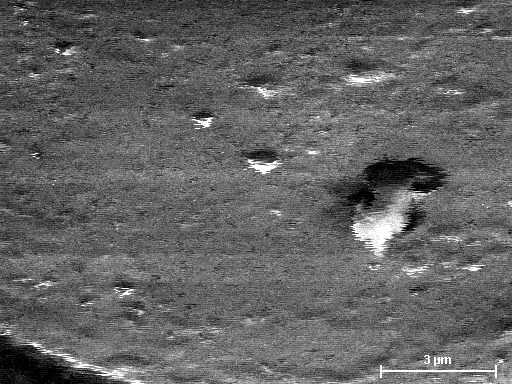
\includegraphics[width=.8\textwidth]{raw/SEM/Hummelauge_M9010}
			\subcaption{}
			\label{fig:Hummelaugex9010}
		\end{subfigure}
		\begin{subfigure}[c]{.45\textwidth}
			\centering
			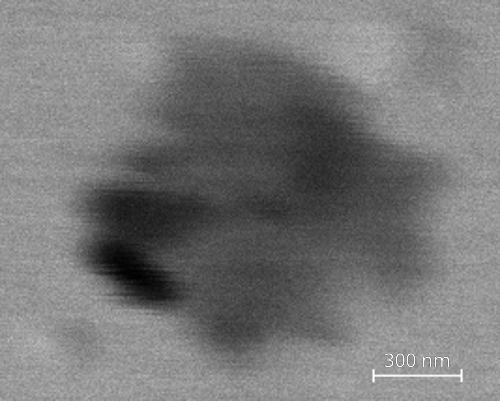
\includegraphics[width=.8\textwidth]{raw/SEM/45kresolutionExt2.png}
			\subcaption{}
			\label{fig:45k}
		\end{subfigure}
		\caption{(a) SEM-Bild eines Hummelauges bei einer Vergrößerung von x9010.\\
		(b) SEM-Bild einer für diesen Versuch hergestellten Probe bei einer Vergrößerung von x45000.
		}
		\label{fig:resolution}
	\end{figure}
	Bei einem Vergrößerungsfaktor von über $9000$ liegen diese Strukturen im \SI{1}{\micro\meter}-Bereich.
	Zum Vergleich mit geringeren Vergrößerungen dient \cref{fig:Hummelauge} im Anhang.

	\

	Um noch kleinere Strukturen mit dem SEM darzustellen, werden die für diesen Versuch hergestellten Proben verwendet.
	Lassen die Goldcluster sich auflösen, so bedeutet dies, dass die Auflösungsgrenze des SEMs in den \SI{10}{\nano\meter}-Bereich reicht.
	\cref{fig:45k} zeigt die kleinste darstellbare Struktur auf dem Kohlenstoffhintergrund der Probe.
	Goldcluster lassen sich nicht erkennen und vermutlich handelt es sich auch hier um Schmutz.
	Dennoch kann durch den Kontrast an der dunkleren Stelle mit dem umliegenden Gebiet eine Struktur im \SI{300}{\nano\meter}-Bereich erkannt werden.

	% TODO noch iwie 1-2 Sätze zum Abschluss? dunno

\subsection{Untersuchung einer Messingprobe}

	Die zu untersuchende Messingprobe befindet sich wie auch die Kupfer- und die Zinkprobe an verschiedenen Stellen der gleichen Halterung.
	Dies ist in \cref{fig:messing_halterung} dargestellt.
	\begin{wrapfigure}{r}{.5\textwidth}
		\centering
		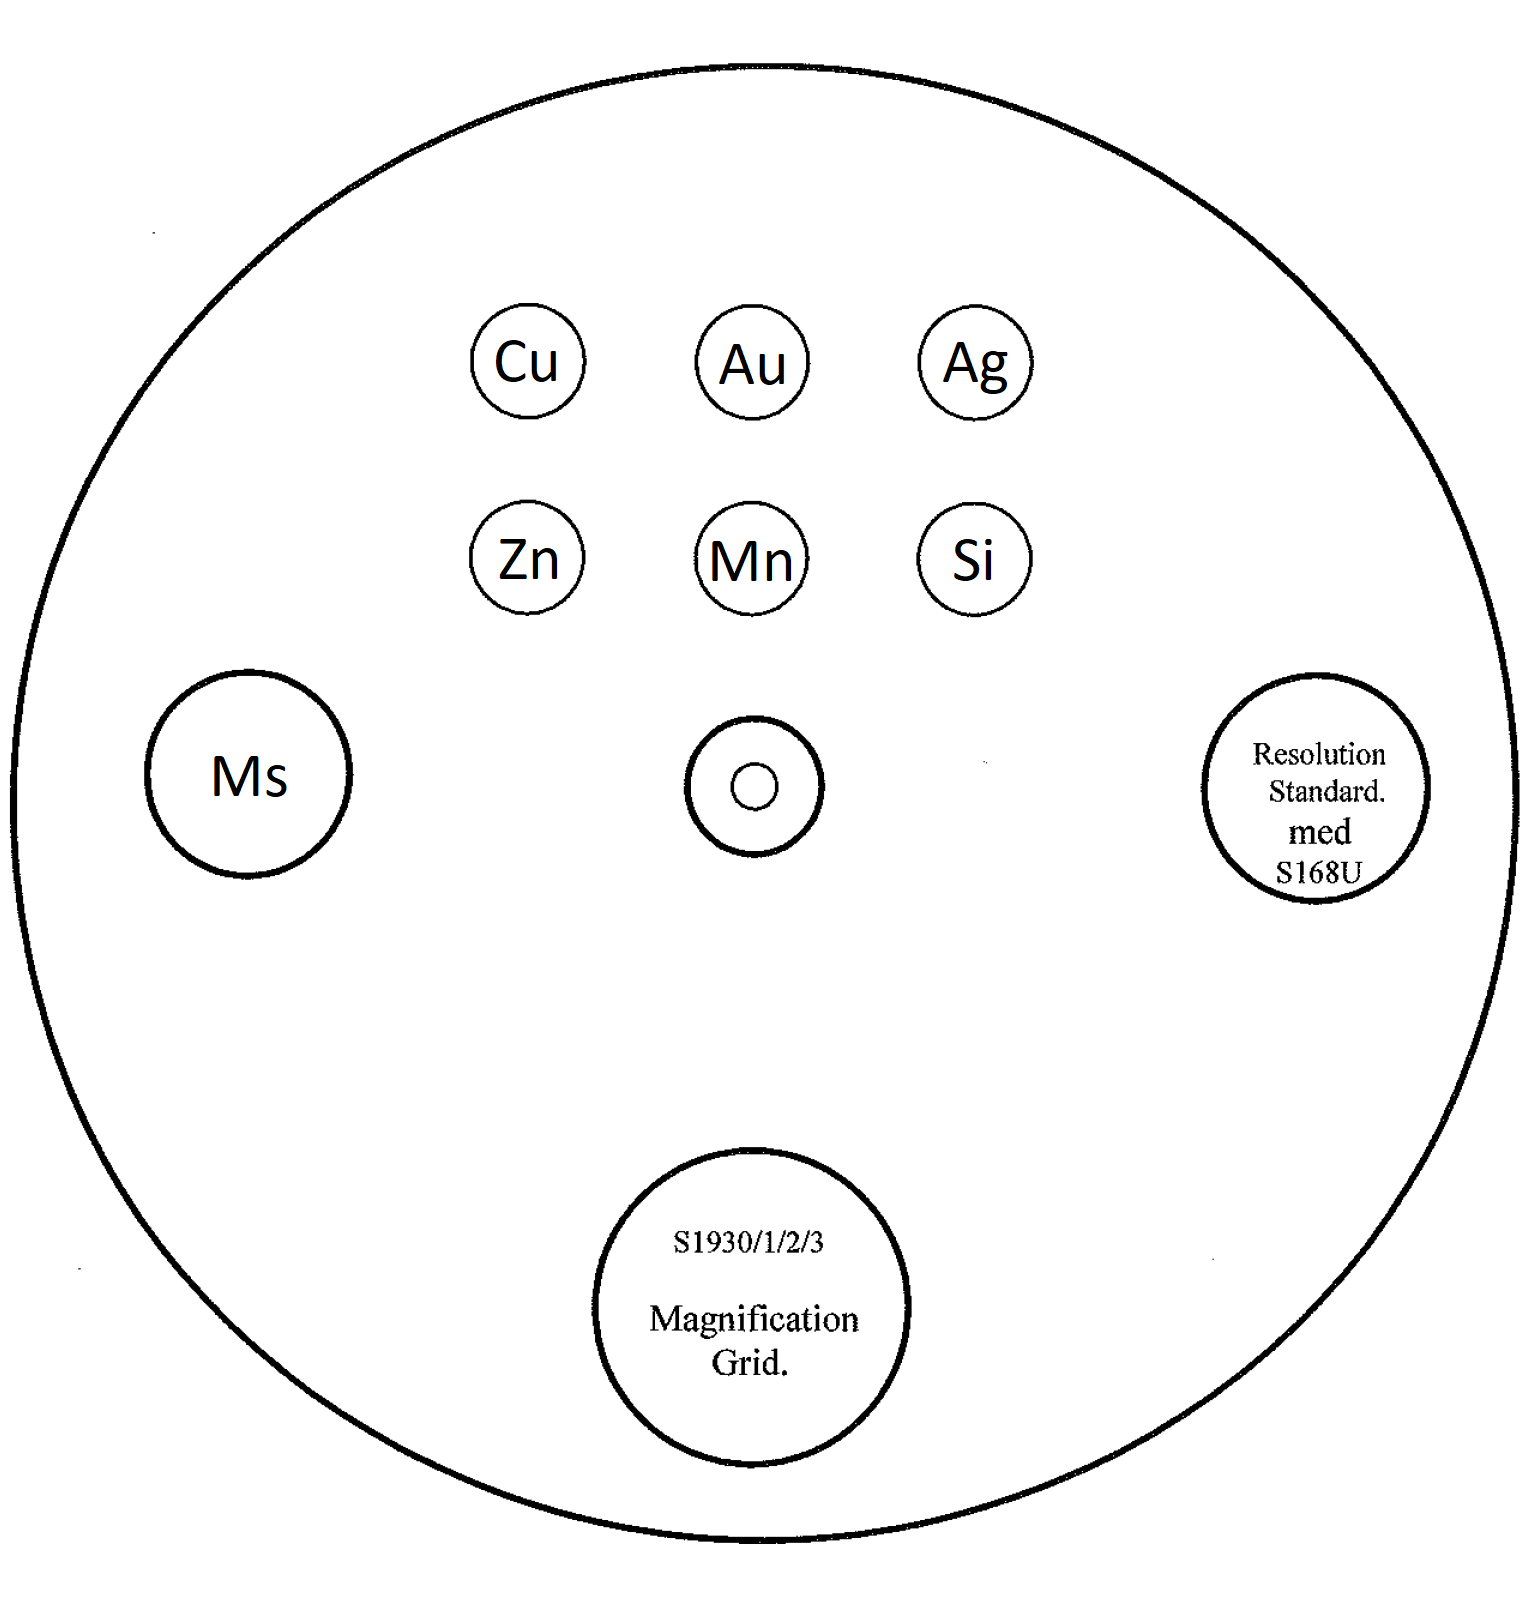
\includegraphics[width=.4\textwidth]{img/Messingprobe}
		\caption{Schematische Darstellung der Halterung mit unterschiedlichen Proben.\cite{wwu}}
		\label{fig:messing_halterung}
	\end{wrapfigure}
	Um nur das Röntgen-Absorptionsspektrum einer bestimmten Probe aufzunehmen, wird nur der Bereich, welcher von Interesse ist, abgebildet.
	Dafür wird die zu untersuchende Probe innerhalb des Mikroskops in den Mittelpunkt des Elektronenstrahls gefahren und die Vergrößerung erhöht, damit nur eine Legierung bzw. ein Element sichtbar ist.

	\

	In \cref{fig:messing_spektrum} sind die aufgenommen Spektren für Messing, Kupfer und Zink zu erkennen.
	Da für die Bestimmung von Kupfer- und Zinkgehalt hier nur die charakteristischen $K_\alpha$- und $K_\beta$-Linien relevant sind, sind die gesamten Spektren und Darstellungen der $L$-Linien (\cref{fig:l-linien}) dem Anhang zu entnehmen.
	Letztere sind für die Auswerung nicht geeignet, da dort nicht zwischen $L_\alpha$ und $L_\beta$ unterschieden werden kann.

	Die Verteilung der Datenpunkte um die $K$-Linien werden als gaußförmig angenommen und daher mit Gauß-Funktionen angenähert.
	Als Startparameter dienen die von \cite{brukerPTE} gegebenen Energien für die $K$-Linien von Kupfer und Zink.
	Dargestellt ist dies in \cref{fig:k-linien}.
	\begin{figure}[ht]
		\centering
		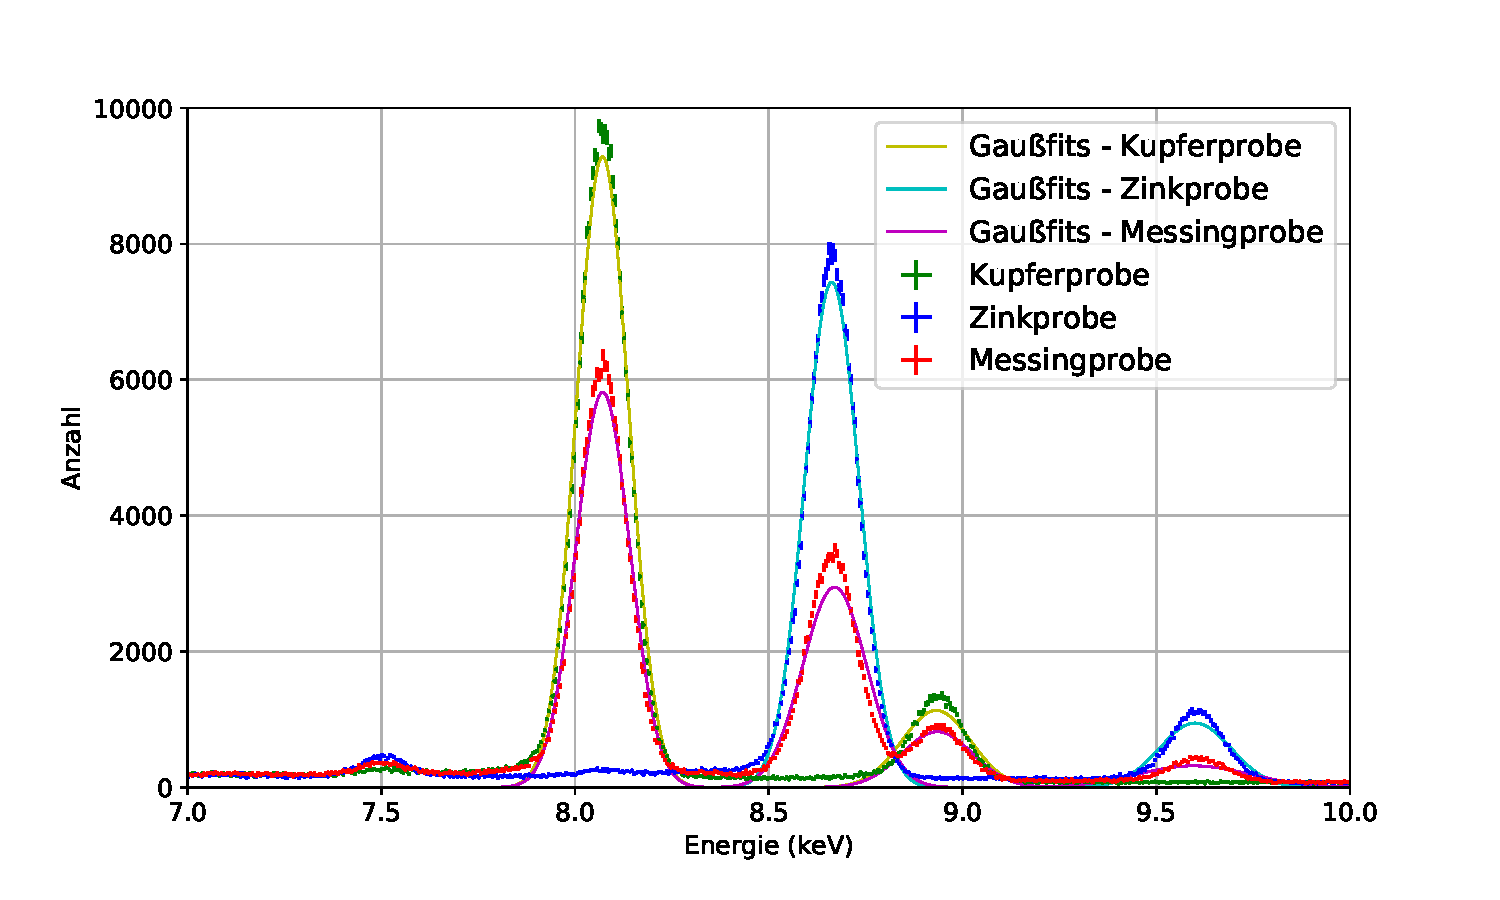
\includegraphics[width=.8\textwidth]{plots/KupferprobeK}
		\caption{Röntgen-Absorptionsspektrum im Bereich der $K$-Linien von Kupfer und Zink für eine Messing-, Kupfer- und Zinkprobe. Zusätzlich dazu Gauß-Fits für die einzelnen Proben und deren charakteristischer Linien.}
		\label{fig:k-linien}
	\end{figure}
	Für die Unsicherheit der Anzahl von $n$ Datenpunkten wird $\sqrt{n}$ verwendet.
	Der direkte Vergleich der Amplituden der Gauß-Fits von Messing zu denen von Kupfer bzw. Zink liefert die in \cref{tab:amplituden} dargestellte Verhältnisse.
	\begin{table}[H]
		\centering
		\caption{Verhältnisse der Amplituden charakteristischer Linien von Messing (Ms) zu Kupfer (Cu) bzw. Zink (Zn).}
		\begin{tabular}{l|c|c|c}
			Verhältnis & $K_\alpha$ & $K_\beta$ & Mittelwert \\ \hline
			% & & & \\
			Ms/Cu & $(62.6\pm3.5)\%$ & $(72.0\pm9.0)\%$ & $(67.0\pm5.0)\%$ \\
			Ms/Zn & $(39.6\pm2.9)\%$ & $(34.0\pm4.0)\%$ & $(36.6\pm2.5)\%$ \\
		\end{tabular}
		\label{tab:amplituden}
	\end{table}

\subsection{Untersuchung unbekannter Elemente}

	Für die letzte SEM-Messung wird die Probe mit den vier unbekannten Elementen eingesetzt.
	Um die Elemente zu bestimmen wird zunächst ein Bild von jedem Quadranten aufgenommen und das zugehörige Röntgen-Absorptionsspektrum betrachtet.
	Die Software von Bruker ermöglicht einen direkten Vergleich der aufgenommenen Spektren mit den Absorptionslinien einer Vielzahl an Elementen.
	Die größte Übereinstimmungen ergeben sich bei den Elementen Aluminium, Kupfer, Silber und Kohlenstoff.

	Um eine Karte der Elemente anzufertigen, wird ein Bild der Probenmitte aufgenommen.
	Bei jedem Rastervorgang wird pro Position ein Spektrum aufgenommen und direkt mit den ausgewählten Elementen verglichen.
	Wie in \cref{fig:bunteMap} dargestellt, nimmt ein Pixel bei Übereinstimmung die Farbe des jeweiligen Elements an.
	\begin{figure}[H]
		\centering
		\begin{subfigure}[c]{.45\textwidth}
			\centering
			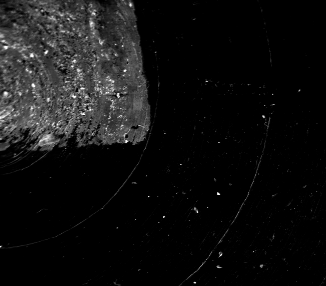
\includegraphics[width=.8\textwidth]{raw/SEM/Map4ProbenExt}
			\subcaption{}
			\label{fig:farbloseMap}
		\end{subfigure}
		\begin{subfigure}[c]{.45\textwidth}
			\centering
			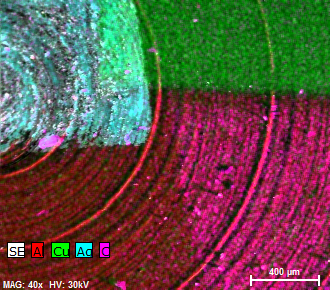
\includegraphics[width=.8\textwidth]{raw/SEM/Mapdaten4Proben}
			\subcaption{}
			\label{fig:bunteMap}
		\end{subfigure}
		\caption{(a) SEM-Bild der Proben mit den unbekannten Elementen.
		(b) SEM-Bild mit Elementkarte aus den Röntgen-Absorptionsspektren von Silber, Kupfer, Aluminium und Kohlenstoff.}
		\label{fig:elementalMap}
	\end{figure}
	Ohne die Röntgenanalyse lassen sich drei der Quadranten, wie in \cref{fig:farbloseMap} zu sehen, nicht unterscheiden.

\subsection{Diskussion der SEM-Ergebnisse}

	Zur Bestimmung der Auflösungsgrenze wurden verschiedene Proben untersucht.
	Die bestmögliche Auflösung lag im \SI{300}{\nano\meter}-Bereich.

	\

	Durch Mittlung ergab sich für den Kupfergehalt im Messing ein Wert von $(67.0\pm5.0)\%$ und für den Zinkgehalt $(36.6\pm2.5)\%$.
	Als Angabe für das Messing wurde "duplex brass" von \cite{wwu} verwendet.
	Nach \cite{wikiMs} entspricht dies Messing mit einem Kupfergehalt von 55\% bis 65\% und dementsprechend einen Zinkgehalt von 35\% bis 45\%.
	Damit liegt über die hier ermittelten Werte eine Übereinstimmung innerhalb einer Unsicherheit vor.
	Ein tatsächliches Verhältnis von ~65\% Kupfer zu ~35\% liegt nahe.
	Es sei angemerkt, dass die getrennte Betrachtung der unterschiedlichen $K$-Linien eine größere Übereinstimmung für die $\alpha$- und eine geringere für die $\beta$-Linen mit sich trägt.
	Dass die Anzahl der Datenpunkte bei den $\beta$-Linen deutlich geringer war, könnte eine mögliche Begründung dafür sein, weswegen bei einer längeren Messung möglicherweise ein besseres Ergebnis erzielt werden könnte.

	\

	Der letzte Punkt der SEM-Auswertung befasste sich mit der Erstellung der Elementkarte.
	Hier ließen sich die vier unbekannten Elemente zu Silber, Kupfer, Aluminium und Kohlenstoff bestimmen.
	Der direkte Vergleich zwischen SEM-Bild ohne und mit der Elementkarte in \cref{fig:elementalMap} unterstützt dies.
	Ohne die Elementkarte sticht nur ein Element hervor.
	Aus der Röntgenanalyse folgt, dass es sich dabei um Silber handelt.
	Dies erscheint sinnvoll, da Silber von den vier Elementen die höchste Elektronendichte besitzt und daher im SEM-Bild am hellsten erscheint.
	Weiterhin kann \cref{fig:bunteMap} entnommen werden, dass die Probe eine Aluminiumbasis besitzt, auf die andere Elemente aufgedampft wurden.
	Besonders an dem Kohlenstoffquadranten ist dies ersichtlich, da neben den pinken Pixeln auch rote vorliegen.
	Ebenso grenzt der Kupferquadrant nicht direkt an den Kohlenstoff, sondern es befindet sich noch Aluminium dazwischen.

	% TODO noch was?

	\newpage
\section{TEM} % TODO

 Es wird ein Libra 200 FE TEM (Zeiss) verwendet, um die in \cref{sec:prep} beschriebenen Proben zu untersuchen.
 Hierbei zeigt sich, dass die durchschnittlich etwa \SI{20}{nm} großen Goldcluster aufgelöst werden können.
 Aufgrund von Problemen mit dem Gerät werden jedoch im Folgenden ältere Messungen von Wolframdiselenid ausgewertet.

 In \cref{fig:tem_dfbf} sind hiermit aufgenommene Hell- und Dunkelfeldbilder dargestellt. %TODO muss man zusätzliuch sagen, dass das kein STEM war oder ist das so klar?
 Für die Hellfeldaufnahme wird in der Streuebene mittels einer Blende alle Strahlen außer des ungestreuten Elektronenstrahls herausgefiltert.
 Dementsprechend werden dickere Strukturen im Bild dunkel sichtbar, während dünne Strukturen heller und Orte ohne Probe am hellsten erscheinen.

 Für die Dunkelfeldaufnahme wird stattdessen einer der gebeugten Spots in der Streuebene ausgewählt.
 Hierdurch erscheinen besonders stark streuende, also dicke, Strukturen heller.

	\begin{figure}[H]
		\centering
	\begin{subfigure}[b]{0.45\textwidth}
				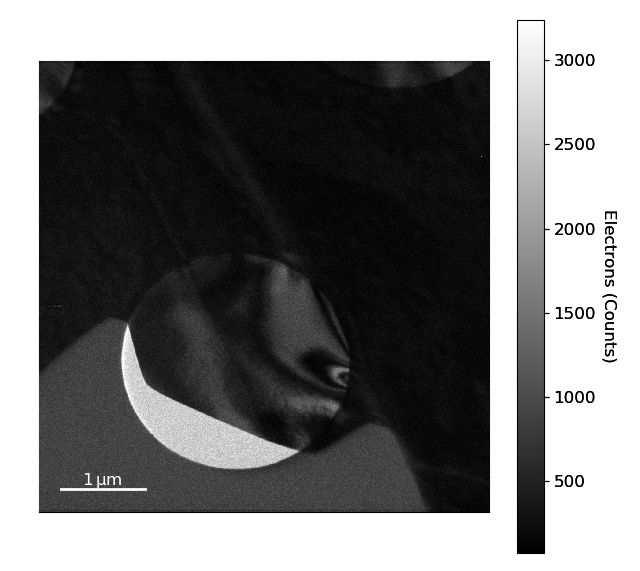
\includegraphics[width= 1 \linewidth]{img/tem_bf}
				\caption{Hellfeld}
		\end{subfigure}
	\begin{subfigure}[b]{0.45\textwidth}
				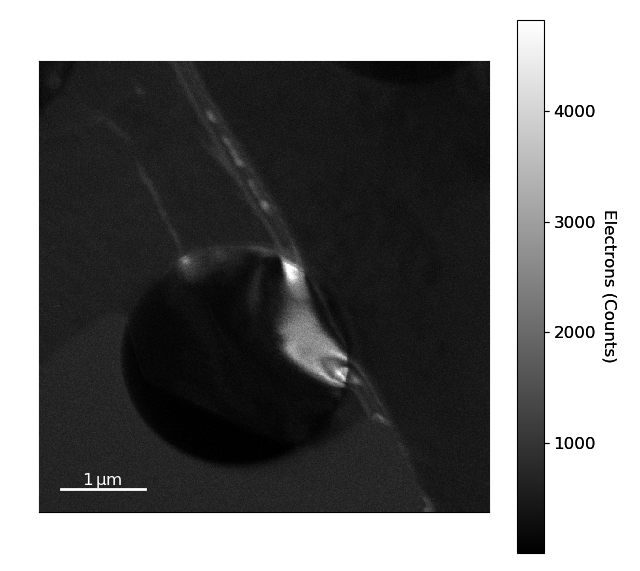
\includegraphics[width= 1 \linewidth]{img/tem_df}
				\caption{Dunkelfeld}
		\end{subfigure}
		\caption{
      Hell- und Dunkelfeld-Aufnahmen im TEM. Die runde Form ist ein Loch im membranartigen Probenhalter. Im Hellfeld ist der WSe$_2$-Kristall über dem Loch in dunkler Farbe erkennbar. Im Dunkelfeld ist in heller Farbe sichtbar, wo der Kristall besonders dick ist.
				}
    \label{fig:tem_dfbf}
	\end{figure}



 \subsection{Bestimmung der Atomabstände in der Projektionsebene}

 In \cref{fig:hrtem} ist die Aufnahme der Oberfläche des Kristalls dargestellt.
 Daraus wird durch Abzählen der Täler im Linienprofil die Atomabstände in den beiden sichtbaren Richtungen bestimmt und in \cref{tab:netz} dargestellt.
 Die Unsicherheit wurde mit einer Abweichung in Höhe von einem Atomabstand über die abgezählte Täler abgeschätzt.

	\begin{figure}[H]
		\centering
	\begin{subfigure}[b]{0.40\textwidth}
        \centering
				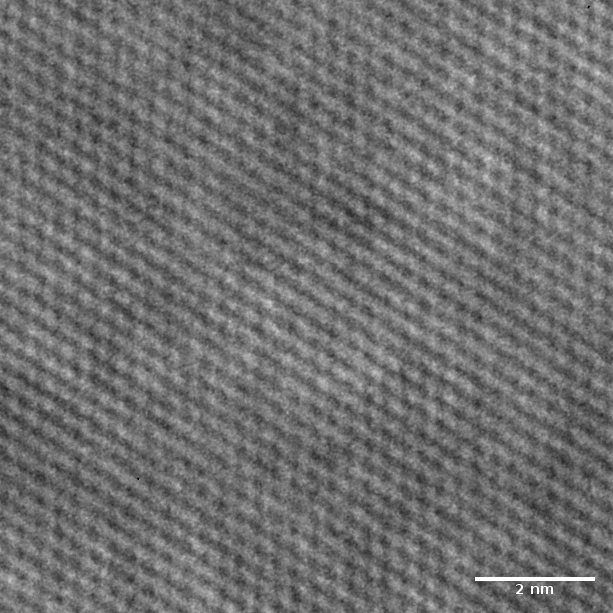
\includegraphics[width= 1 \linewidth]{img/hrtem_zoomzoom}
				\caption{}
        \label{fig:hrtem_img}
		\end{subfigure}

	\begin{subfigure}[b]{0.65\textwidth}
        \centering
				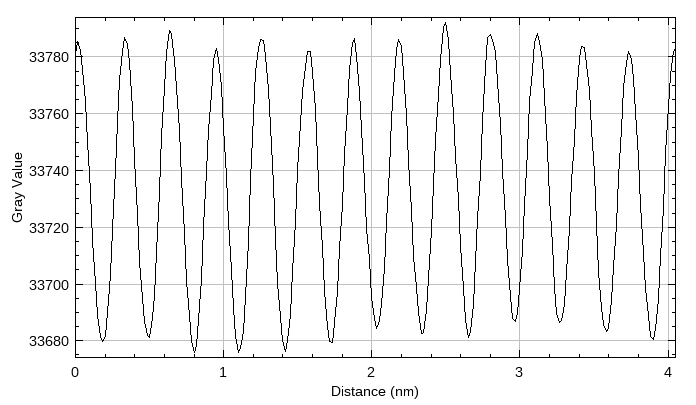
\includegraphics[width= 1 \linewidth]{img/tem_line-Plot_hrtem_orig}
				\caption{}
		\end{subfigure}
		\caption{
      TEM-Aufnahme der Oberfläche des WSe$_2$-Kristalls und eines der Linienprofile. Für dieses wurde über mehrere parallele Atomreihen gemittelt, wodurch das Rauschen stark verringert wurde.
				}
    \label{fig:hrtem}
	\end{figure}

  Für \cref{fig:ft} wurde diese Aufnahme (mit geringerer Vergrößerung als in \cref{fig:hrtem_img}) fouriertransformiert.
  Darin tauchen räumliche Frequenzen (die Gitterstruktur) als helle Punkte auf.
  Aus der Position dieser Punkte ergibt sich die räumliche Wellenlänge, die hier dem Atomabstand entspricht.
  Die so ermittelten Atomabstände sind in \cref{tab:netz} eingetragen.
  Für die Unsicherheit wurde die FWHM der räumlichen Peaks verwendet.

	\begin{figure}[H]
  \centering
			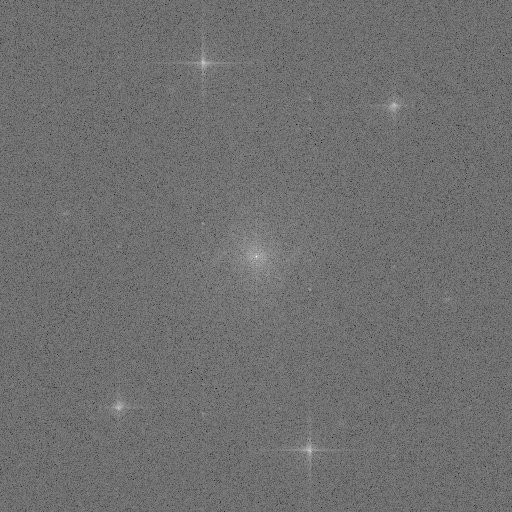
\includegraphics[width= 0.4 \linewidth]{img/tem_hrtem_crop_fft}
			\caption{
        Räumliche Fouriertransformation der TEM-Aufnahme in \cref{fig:hrtem}.
			}
			\label{fig:ft}
	\end{figure}

  Als letzte Methode wird das Bild in der Streuebene bei Beleuchtung einer hinreichend großen Fläche (einige Atomabstände) aufgenommen und in \cref{fig:diff} abgebildet.
  Anhand der Abstände der Spots wird über den Kehrwert die Atomabstände des Realraumgitters (in der Projektion auf eine Ebene) bestimmt und in \cref{tab:netz} vermerkt.
  Es wird der Abstand über mehrere Spots gemessen und gemittelt.

	\begin{figure}[H]
  \centering
			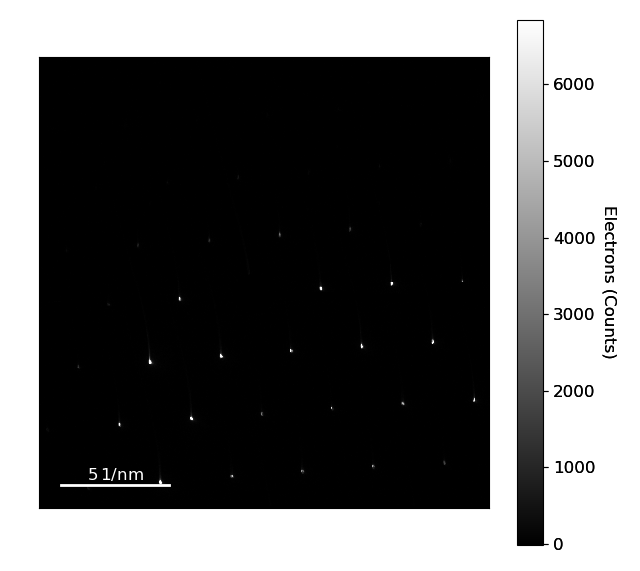
\includegraphics[width= 0.6 \linewidth]{img/tem_diff}
			\caption{
        TEM-Aufnahme in der Streuebene.
			}
			\label{fig:diff}
	\end{figure}



	\begin{table}
		\centering
		\caption{Auf unterschiedliche Arten bestimmte Atomabstände der WSe$_2$-Probe. Die Richtungen können sind nur zu Unterscheidung innerhalb der selben Messmethode angegeben. Zwischen den Methoden sind die Richtungen nicht konstant.
    Für den Literaturwert wurde der Abstand zwischen den Selenatomen angegeben.}
		\begin{tabular}{c| c | c}
			Methode & Richtung & Atomabstand \\ \hline
			% & & & \\
      Linienprofil &  1 & \SI{0.31 \pm 0.01}{nm}\\
      Linienprofil &  2 & \SI{0.31 \pm 0.01}{nm}\\
      Fouriertransformation & 1 & \SI{0.29 \pm 0.01}{nm}\\
      & 2 & \SI{0.3 \pm 0.01}{nm}\\
      Streuebene & 1 & \SI{0,312 \pm 0.001}{nm} \\
      & 2 & \SI{0,317 \pm 0.001}{nm} \\
      & 3 & \SI{0,314 \pm 0.001}{nm} \\
      Mittelwert & & \SI{0,308 \pm 0.002}{nm}\\
      Literatur & & \SI{0,334}{nm} \cite{wiki_wse}\\
		\end{tabular}
		\label{tab:netz}
	\end{table}

\subsection{Diskussion der TEM-Ergebnisse}

  Die mittels der verschiedenen Messmethoden ermittelten Atomabstände in \cref{tab:netz} stimmen innerhalb der Messunsicherheit miteinander überein.
  Dass abhängig von der Messrichtung kein Unterschied im Atomabstand besteht, stimmt mit der zu erwartenden hexagonalen Symmetrie innerhalb einer Wolframdiselenidlage überein.
  Die Abweichung nach Unten gegenüber dem Literaturwert für den Abstand der Selenatome kommt dadurch zustande, dass nicht dieser Abstand, sondern der Abstand der Projektion der Atome (Wolfram und Selen) auf eine ebene Fläche gemessen wurde.
  Wie in \cref{fig:strukt} zu sehen ist, liegen auch innerhalb einer Monolage nicht alle Atome in einer Ebene.

	\begin{figure}[H]
  \centering
			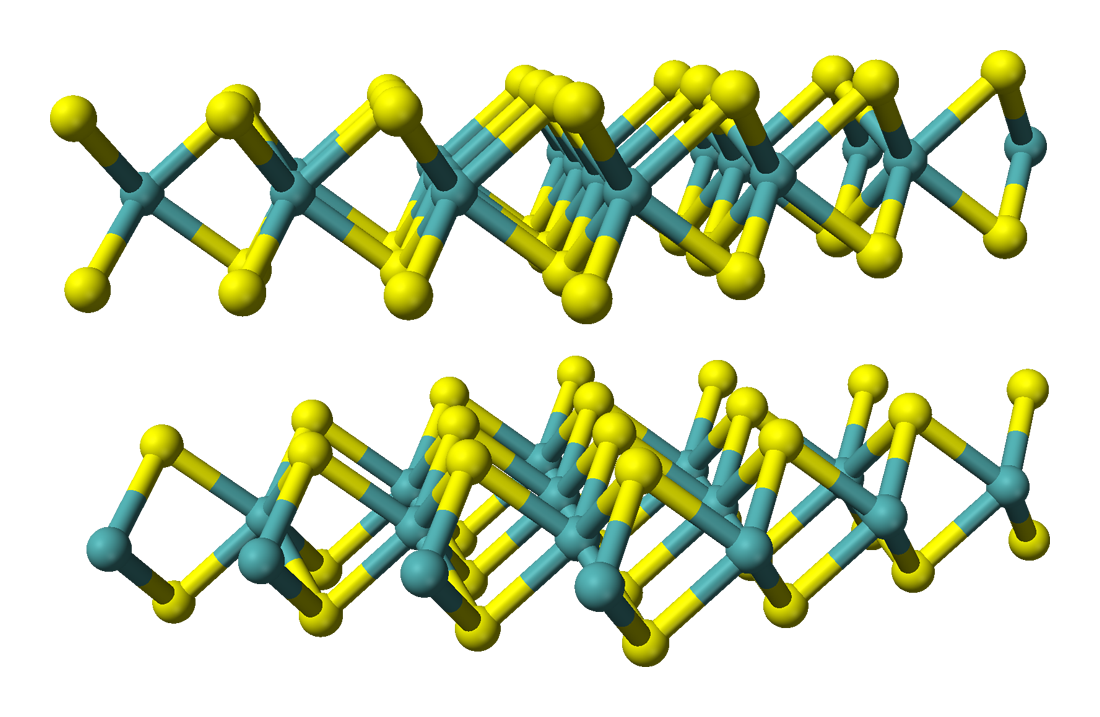
\includegraphics[width= 0.4 \linewidth]{img/strukt}
			\caption{
        Struktur einer Monolage Wolframdiselenid. \cite{wiki_wse_bild}
			}
			\label{fig:strukt}
	\end{figure}

  \subsection{EELS}

	\begin{figure}[H]
		\centering
	\begin{subfigure}[b]{0.45\textwidth}
				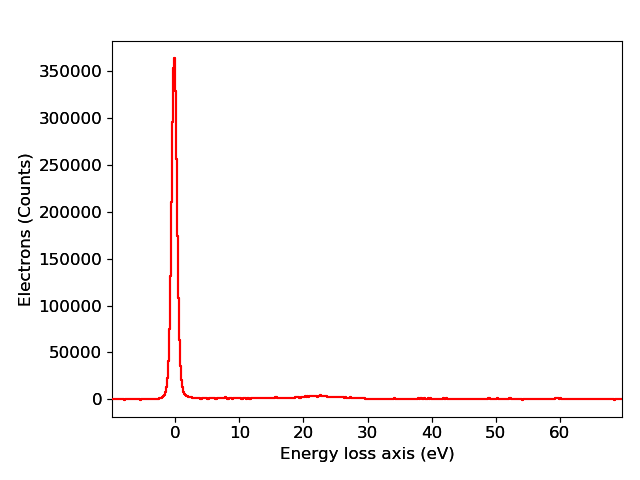
\includegraphics[width= 1 \linewidth]{img/tem_zeroloss}
				\caption{zero-loss}
	\end{subfigure}
	\begin{subfigure}[b]{0.45\textwidth}
				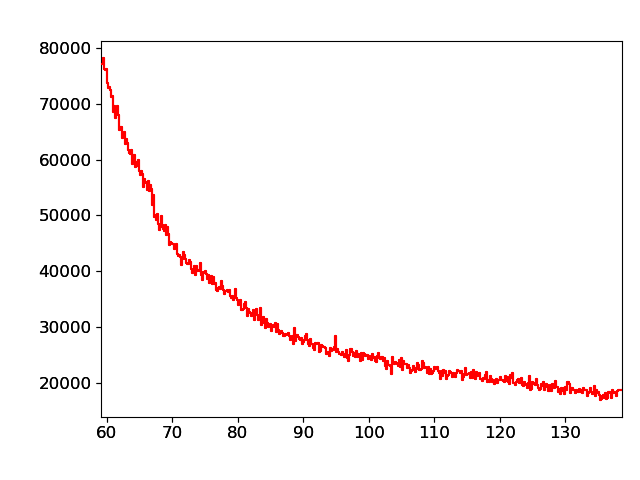
\includegraphics[width= 1 \linewidth]{img/tem_coreloss}
				\caption{core-loss}
	\end{subfigure}
	\begin{subfigure}[b]{0.7\textwidth}
				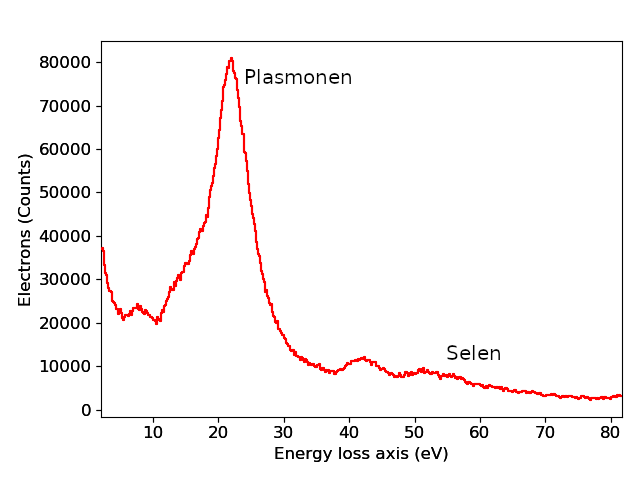
\includegraphics[width= 1 \linewidth]{img/tem_mark}
				\caption{low-loss}
	\end{subfigure}
		\caption{
      EELS-Spektren der Wolframdiselenidprobe.
			}
    \label{fig:eels}
	\end{figure}

  Zuletzt wird das EEL-Spektrum der Probe aufgenommen.
  Es ist in \cref{fig:eels} zu sehen.
  Hier wurden die deutlich erkennbaren Peaks entsprechend ihres Ursprungs beschriftet.
  Wolfram hat lediglich Kanten im Bereich von über \SI{1800}{eV}, also außerhalb des Messbereichs, und eine O-Kante bei \SI{36}{eV} \cite{eelsinfo}, die jedoch im Spektrum aufgrund ihrer geringen Intensität und hohen Ausgeschmiertheit nicht zu erkennen ist.

  Selen besitzt zwei Kanten über \SI{1400}{eV}, die ebenfalls nicht mehr im Messbereich sind.
  Die M$_4,5$-Kante bei \SI{57}{eV} ist jedoch erkennbar.

  Außerdem ist der Plasmonenpeak im Low-Loss-Bereich zu erkennen.
  Im Core-Loss-Bereich sind keine Peaks sichtbar, was anhand der für Wolfram und Selen auf Basis von \cite{eelsinfo} bekannten Kanten der Erwartung entspricht.
  %TODO Der kleine Peak dazwischen passt irgendwie zu nichts.


 %die Multimap-Dateien sind EFTEM-Aufnahmen. Da sollen wir denke nichts mit machen

	% Bezug/Nutzen oder sonst was
	% auch hier die Hypothese wiederholen
	% keine Messwerte hier, nach manchen Menschen, zumindest "direkt" erstellte Diagramme net hier, auch wenn Lesbarkeit-bla
	\newpage
\section{Schlussfolgerung}
	% Rückgriff auf Hypothese und drittes Nennen dieser
	% Quellen zitieren, Websiten mit Zugriffsdatum
	% Verweise auf das Laborbuch (sind erlaubt)
	% Tabelle + Bilder mit Beschriftung
	%TODO schauen, ob hier was angepasst werden muss,

	Insgesamt lässt sich sagen, dass die verschiedenen Teilversuche erfolgreich durchgeführt werden konnten.
	Mit dem SEM konnte eine Auflösung von unter \SI{300}{nm} erreicht werden und anhand von EDX-Messungen Elementkonzentrationen in einer Messingprobe und Elementverteilungen in einer geteilten Probe bestimmt werden.
	Womöglich könnte im SEM eine bessere Auflösung durch Optimierung des Strahlengangs erreicht werden.
	Dies könnte beispielsweise durch Anpassung des Linsensystems und der Aberrationskorrekturen erreicht werden.
	Der damit verbundene Zeitaufwand hätte jedoch den Rahmen dieser Untersuchung überstiegen.

	Im TEM konnte eine Auflösung erreicht werden, die die Bestimmung der Abstände von Atomebenen ermöglicht.
	Diese wurden sowohl im Realraumbild als auch im Bild in der Streuebene bestimmt.

	Zuletzt wird das EEL-Spektrum der Probe aufgenommen und Plasmonen- und Selen-Peaks identifiziert.

		% --- Anhang einbinden
	\newpage
\appendix
\section{Appendix}\label{sec:appendix}

\subsection{Uncertainties}\label{sec:uncertainties}

Any uncertainties will be calculated in accordance with GUM.
The equations used for that are seen in (\ref{fig:GUM_combine}) and (\ref{fig:GUM_formula}).
For the calculations the python library "uncertainties" will be used, which follows the guidelines of GUM.
As for the uncertainties of specific parameters the approximation curves of the $y$-uncertainties of those parameters will be regarded and the method of least squares used.
Here the method "scipy.optimize.curve\_fit()" from the uncertainties library is taken.

\begin{figure}[ht]
	\begin{equation*}
	x = \sum_{i=1}^{N} x_i
	;\quad
	\sigma_x = \sqrt{\sum_{i = 1}^{N} \sigma_{x_i}^2}
	\end{equation*}
	\caption{Formel für kombinierte Unsicherheiten des selben Typs nach GUM.}
	\label{fig:GUM_combine}
\end{figure}

\begin{figure}[ht]
	\begin{align*}
	f = f(x_1, \dots , x_N)
	;\quad
	\sigma_f = \sqrt{\sum_{i = 1}^{N}\left(\pdv{f}{x_i} \sigma_{x_i}\right) ^2}
	\end{align*}
	\caption{Formel für sich fortpflanzende Unsicherheiten erster Ordnung nach GUM.}
	\label{fig:GUM_formula}
\end{figure}

%\newpage
%\subsection{weitere Abbildungen}

\newpage
\subsection{SPEs additional figures}
\label{sec:anhang:spe}

\begin{figure}[H]
    \centering
    \begin{subfigure}{0.47\textwidth}
        \centering
        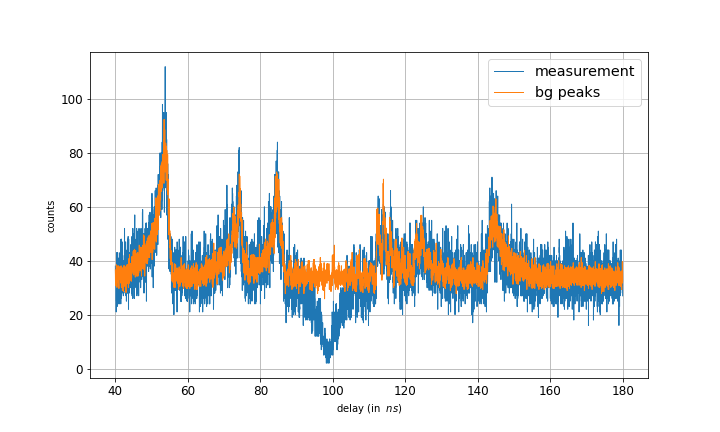
\includegraphics[width=1.0\textwidth]{img/output_t2/50.0muW_bg_peaks.png}
    		\caption{}
    		%\label{fig_antibunch_background_comp}
    \end{subfigure}
    %\hfill
    \begin{subfigure}{0.47\textwidth}
        \centering
        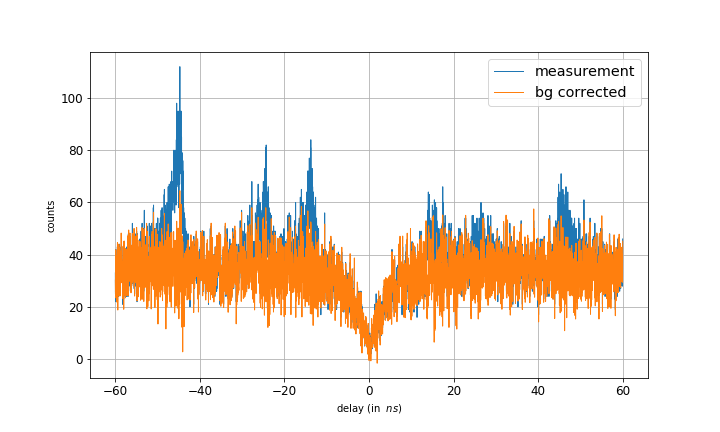
\includegraphics[width=\textwidth]{img/output_t2/50.0muW_bg_vgl.png}
        \caption{}
        %\label{fig_antibunch_raw_corr_comp}
    \end{subfigure}
    \caption{a: Antibunching measurement as recorded and compared to the adjusted background signal. b: Antibunching measurement as recorded and compared to the background corrected signal. The laser power is \SI{50}{\micro W}.} %hoffe ok, dass der eine so doppelt ist
	%\label{fig_antibunch_comp}
\end{figure}
\begin{figure}[H]
    \centering
    \begin{subfigure}{0.47\textwidth}
        \centering
        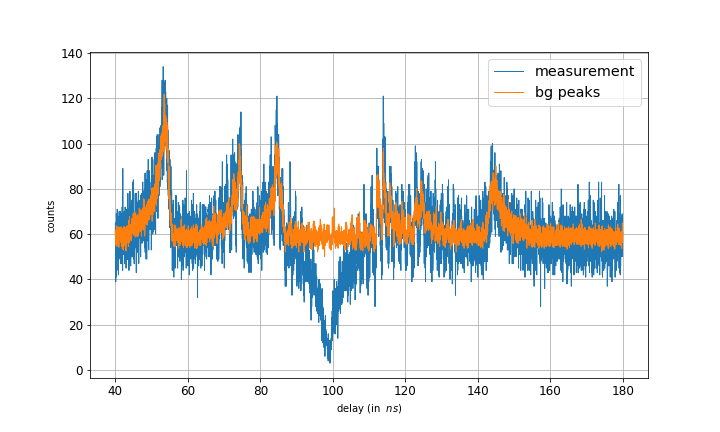
\includegraphics[width=1.0\textwidth]{img/output_t2/100.0muW_bg_peaks.png}
    \caption{}
    %label{fig_antibunch_background_comp}
    \end{subfigure}
    %\hfill
    \begin{subfigure}{0.47\textwidth}
        \centering
        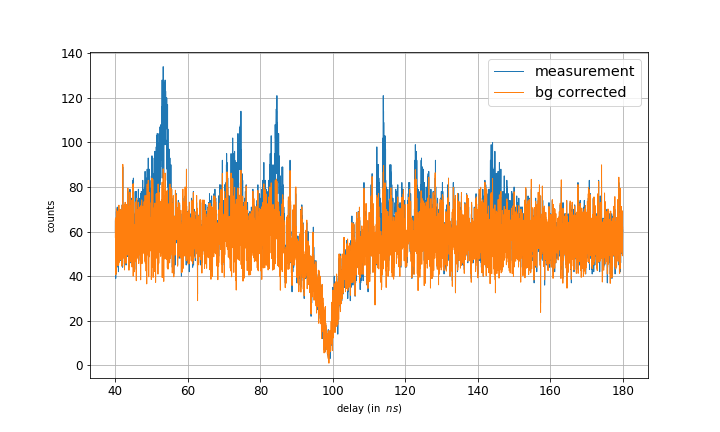
\includegraphics[width=\textwidth]{img/output_t2/100.0muW_bg_vgl.png}
        \caption{}
        %label{fig_antibunch_raw_corr_comp}
    \end{subfigure}
    \caption{a: Antibunching measurement as recorded and compared to the adjusted background signal. b: Antibunching measurement as recorded and compared to the background corrected signal. The laser power is \SI{100}{\micro W}.} %hoffe ok, dass der eine so doppelt ist
	%label{fig_antibunch_comp}
\end{figure}
\begin{figure}[H]
    \centering
    \begin{subfigure}{0.47\textwidth}
        \centering
        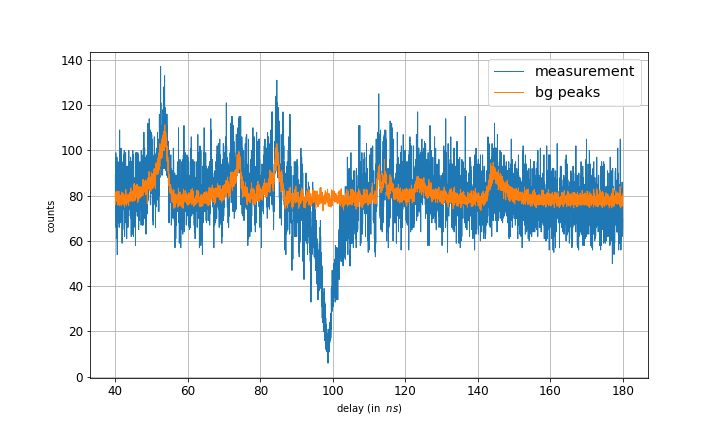
\includegraphics[width=1.0\textwidth]{img/output_t2/250.0muW_bg_peaks.png}
    \caption{}
    %label{fig_antibunch_background_comp}
    \end{subfigure}
    %\hfill
    \begin{subfigure}{0.47\textwidth}
        \centering
        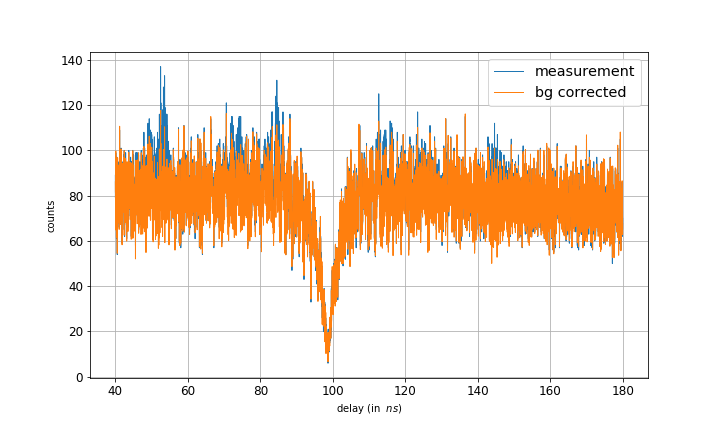
\includegraphics[width=\textwidth]{img/output_t2/250.0muW_bg_vgl.png}
        \caption{}
        %label{fig_antibunch_raw_corr_comp}
    \end{subfigure}
    \caption{a: Antibunching measurement as recorded and compared to the adjusted background signal. b: Antibunching measurement as recorded and compared to the background corrected signal. The laser power is \SI{250}{\micro W}.} %hoffe ok, dass der eine so doppelt ist
	%label{fig_antibunch_comp}
\end{figure}
\begin{figure}[H]
    \centering
    \begin{subfigure}{0.47\textwidth}
        \centering
        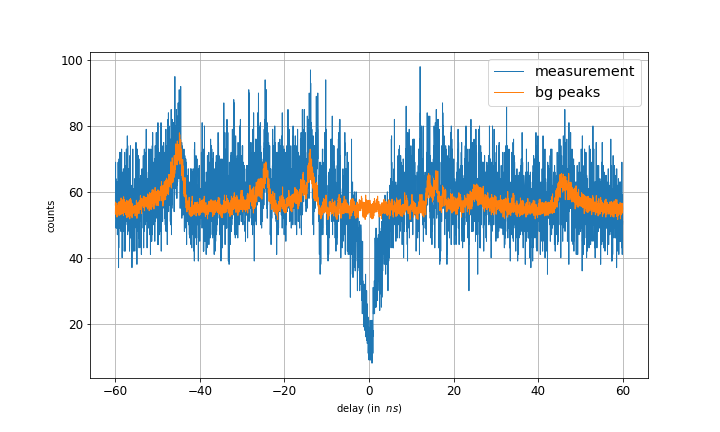
\includegraphics[width=1.0\textwidth]{img/output_t2/500.0muW_bg_peaks.png}
    \caption{}
    %label{fig_antibunch_background_comp}
    \end{subfigure}
    %\hfill
    \begin{subfigure}{0.47\textwidth}
        \centering
        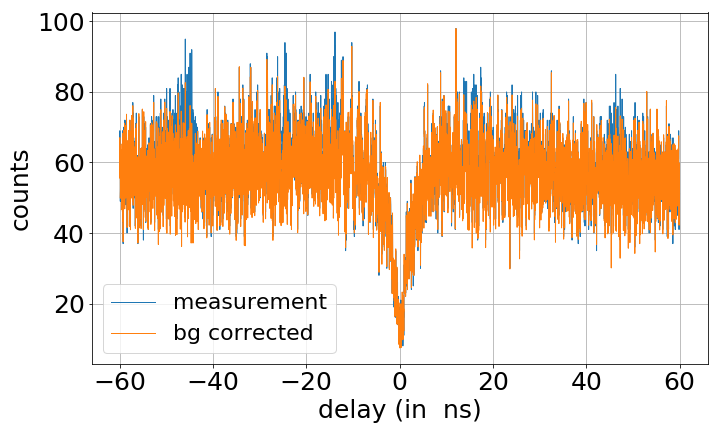
\includegraphics[width=\textwidth]{img/output_t2/500.0muW_bg_vgl.png}
        \caption{}
        %label{fig_antibunch_raw_corr_comp}
    \end{subfigure}
    \caption{a: Antibunching measurement as recorded and compared to the adjusted background signal. b: Antibunching measurement as recorded and compared to the background corrected signal. The laser power is \SI{500}{\micro W}.} %hoffe ok, dass der eine so doppelt ist
	%label{fig_antibunch_comp}
\end{figure}
\begin{figure}[H]
    \centering
    \begin{subfigure}{0.47\textwidth}
        \centering
        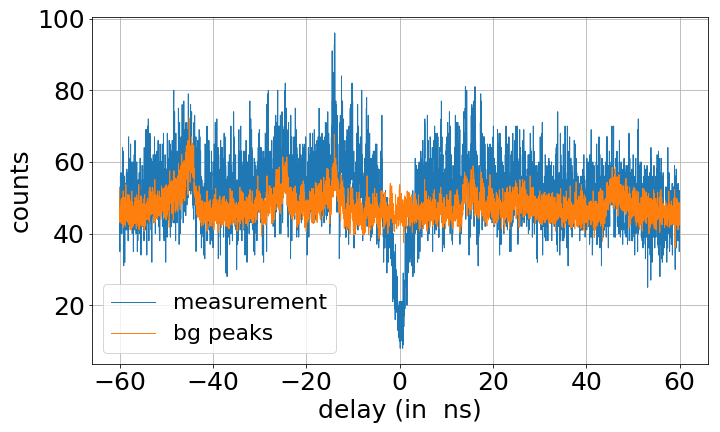
\includegraphics[width=1.0\textwidth]{img/output_t2/1000.0muW_bg_peaks.png}
    \caption{}
    %label{fig_antibunch_background_comp}
    \end{subfigure}
    %\hfill
    \begin{subfigure}{0.47\textwidth}
        \centering
        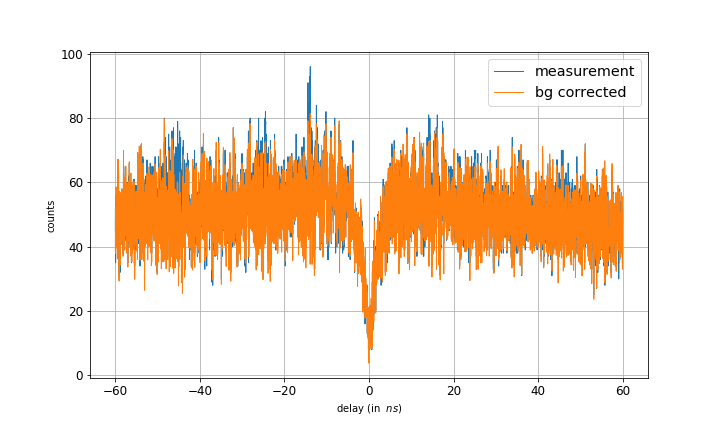
\includegraphics[width=\textwidth]{img/output_t2/1000.0muW_bg_vgl.png}
        \caption{}
        %label{fig_antibunch_raw_corr_comp}
    \end{subfigure}
    \caption{a: Antibunching measurement as recorded and compared to the adjusted background signal. b: Antibunching measurement as recorded and compared to the background corrected signal. The laser power is \SI{1000}{\micro W}.} %hoffe ok, dass der eine so doppelt ist
	%label{fig_antibunch_comp}
\end{figure}
\begin{figure}[H]
    \centering
    \begin{subfigure}{0.47\textwidth}
        \centering
        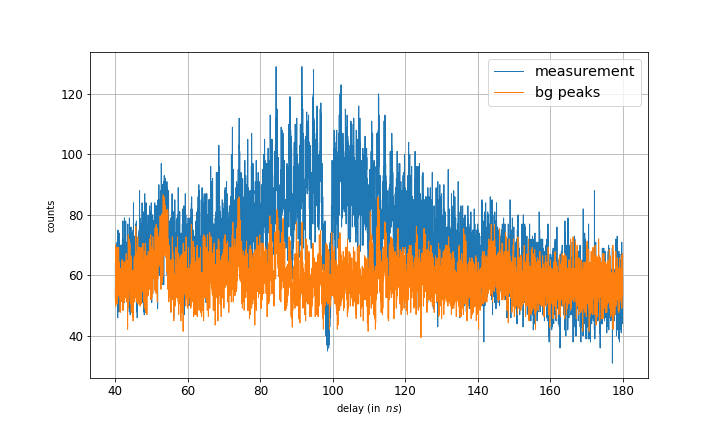
\includegraphics[width=1.0\textwidth]{img/output_t2/2000.0muW_bg_peaks.png}
    \caption{}
    %label{fig_antibunch_background_comp}
    \end{subfigure}
    %\hfill
    \begin{subfigure}{0.47\textwidth}
        \centering
        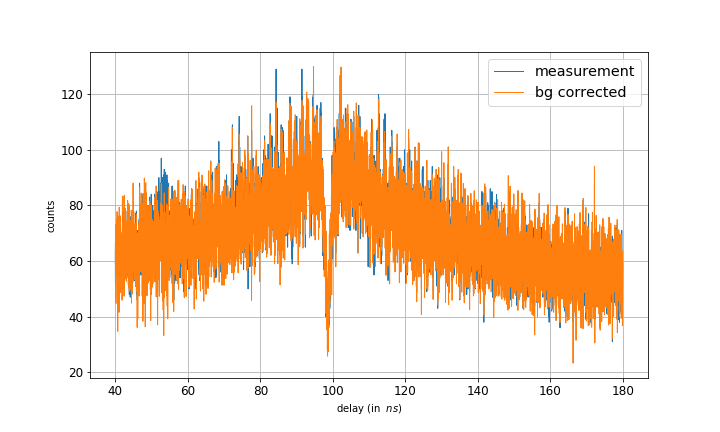
\includegraphics[width=\textwidth]{img/output_t2/2000.0muW_bg_vgl.png}
        \caption{}
        %label{fig_antibunch_raw_corr_comp}
    \end{subfigure}
    \caption{a: Antibunching measurement as recorded and compared to the adjusted background signal. b: Antibunching measurement as recorded and compared to the background corrected signal. The laser power is \SI{2000}{\micro W}.} %hoffe ok, dass der eine so doppelt ist
	%label{fig_antibunch_comp}
\end{figure}

\newpage
\subsection{Faraday Rotation additional figures}
\label{sec:anhang:far}

\begin{figure}[H]
    \centering
    \begin{subfigure}{0.47\textwidth}
        \centering
        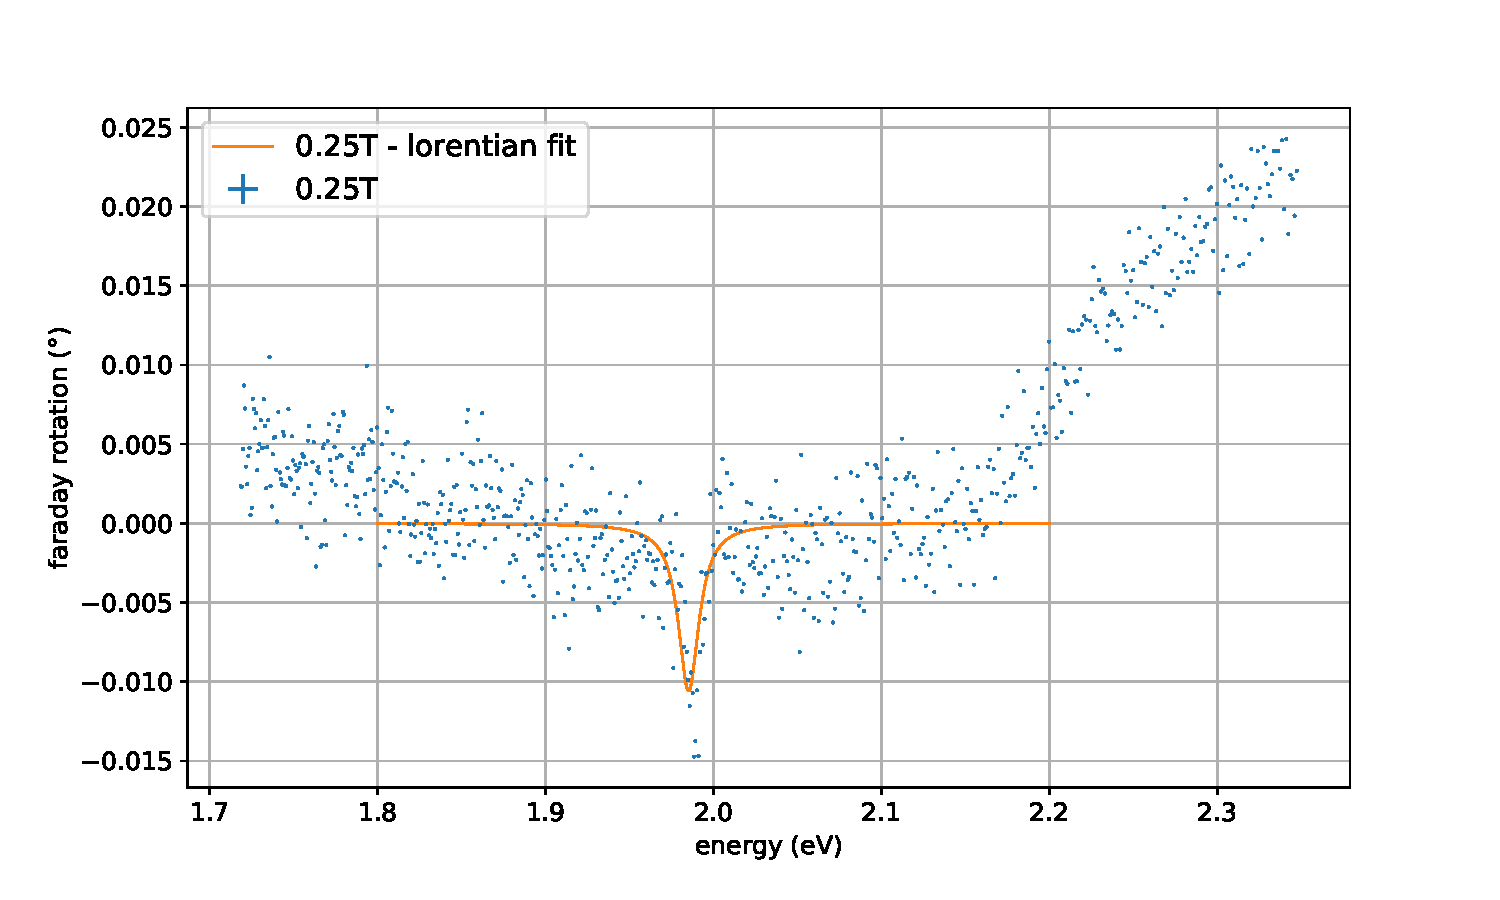
\includegraphics[width=1.0\textwidth]{plots/WS2_250mT.pdf}
    \caption{}
    %label{fig_antibunch_background_comp}
    \end{subfigure}
    %\hfill
    \begin{subfigure}{0.47\textwidth}
        \centering
        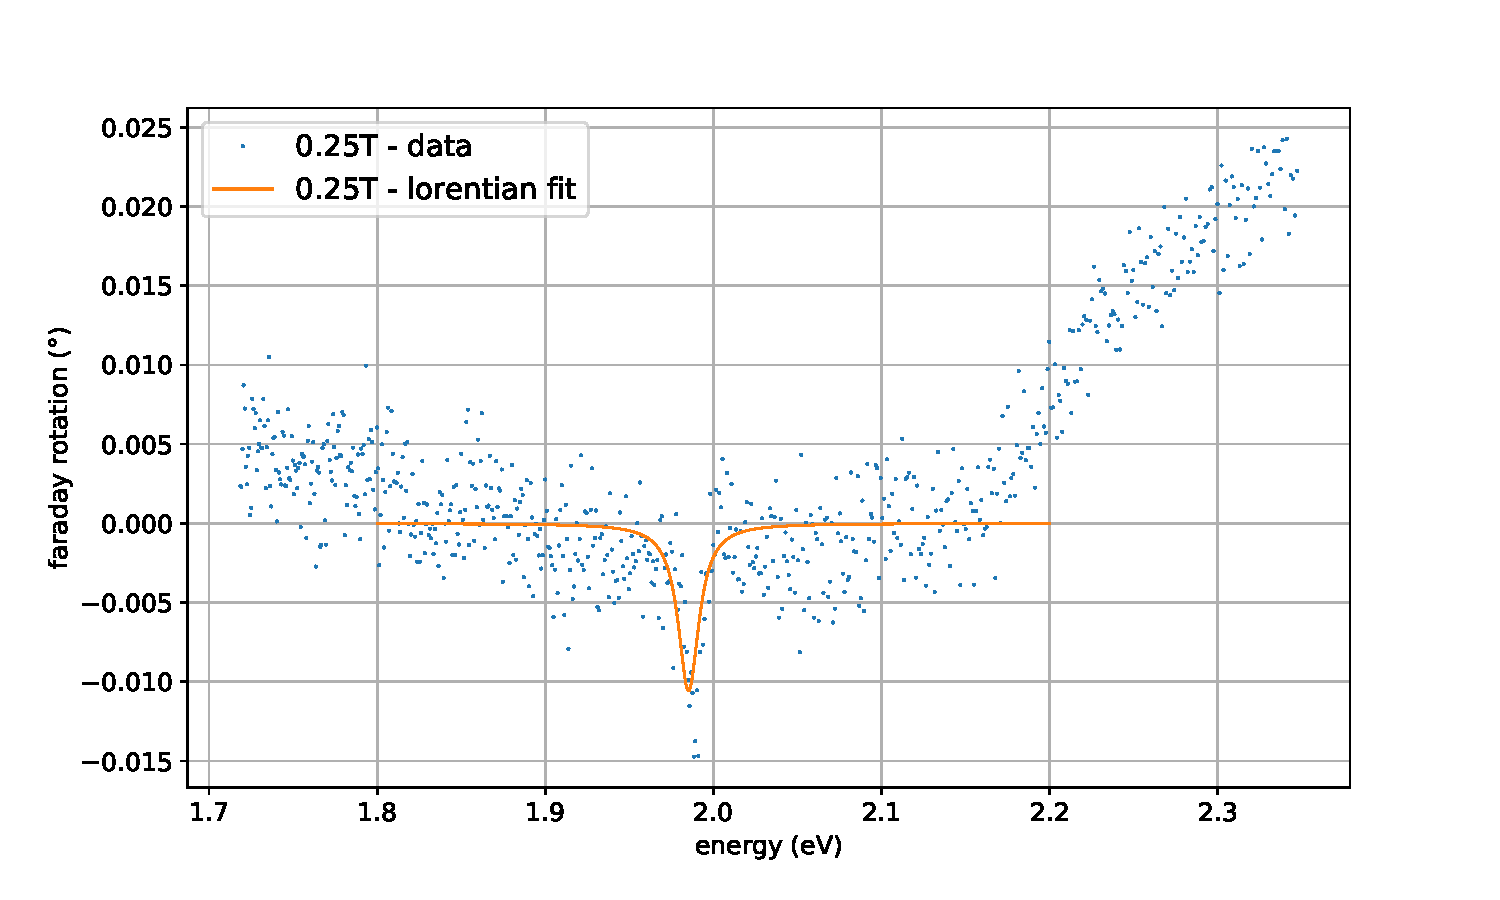
\includegraphics[width=\textwidth]{plots/WS2_250mT_noerror.pdf}
        \caption{}
        \label{fig_WS2_250mT_noerror}
    \end{subfigure}
    \caption{a: Representation of WS$_2$ monolayer data points of the faraday rotation with external magnetic field of \SI{0.25}{\tesla} and lorentian fit. b: Same as a, but without errorbars.} %hoffe ok, dass der eine so doppelt ist
\end{figure}

\begin{figure}[H]
    \centering
    \begin{subfigure}{0.47\textwidth}
        \centering
        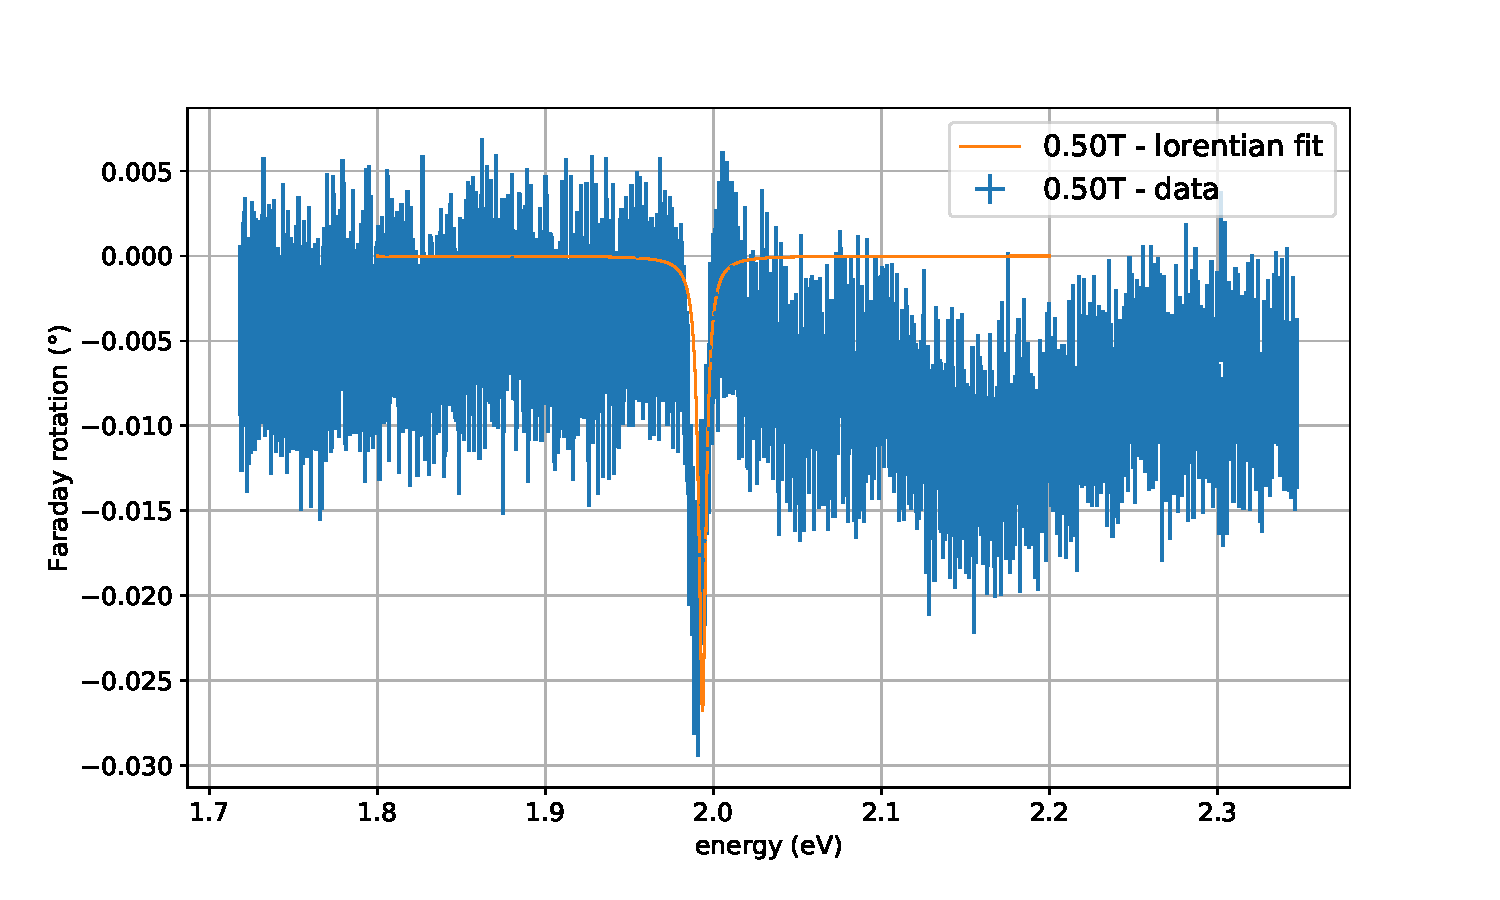
\includegraphics[width=1.0\textwidth]{plots/WS2_500mT.pdf}
    \caption{}
    %label{fig_antibunch_background_comp}
    \end{subfigure}
    %\hfill
    \begin{subfigure}{0.47\textwidth}
        \centering
        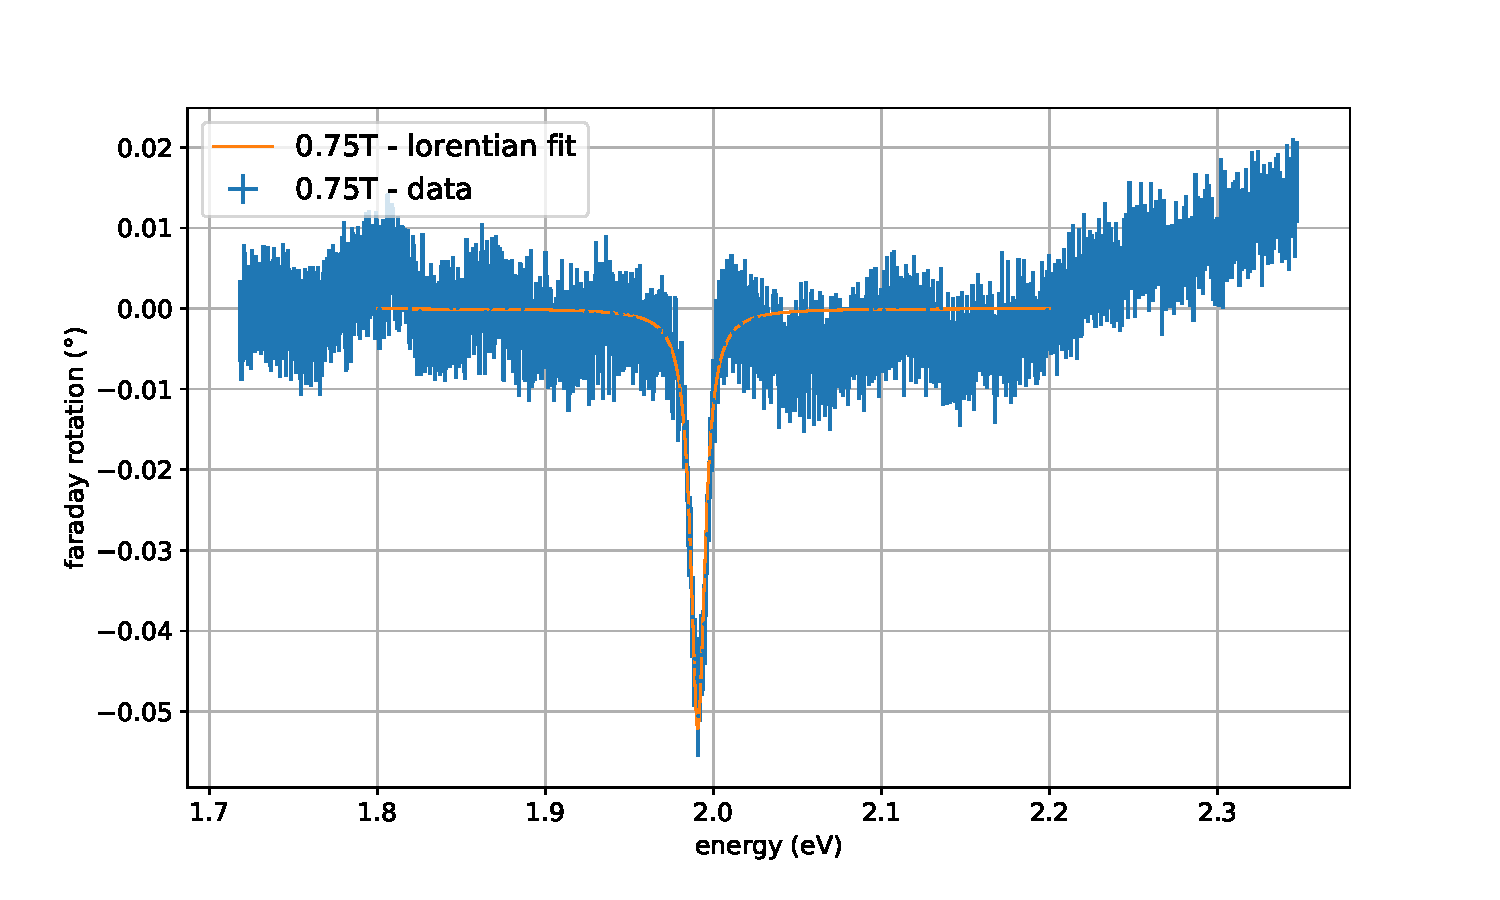
\includegraphics[width=\textwidth]{plots/WS2_750mT.pdf}
        \caption{}
    \end{subfigure}
    \caption{a: Representation of WS$_2$ monolayer data points of the faraday rotation with external magnetic field of \SI{0.50}{\tesla} and lorentian fit. b: Same as a, but at \SI{0.75}{\tesla}.} %hoffe ok, dass der eine so doppelt ist
\end{figure}

\begin{figure}[H]
    \centering
    \begin{subfigure}{0.47\textwidth}
        \centering
        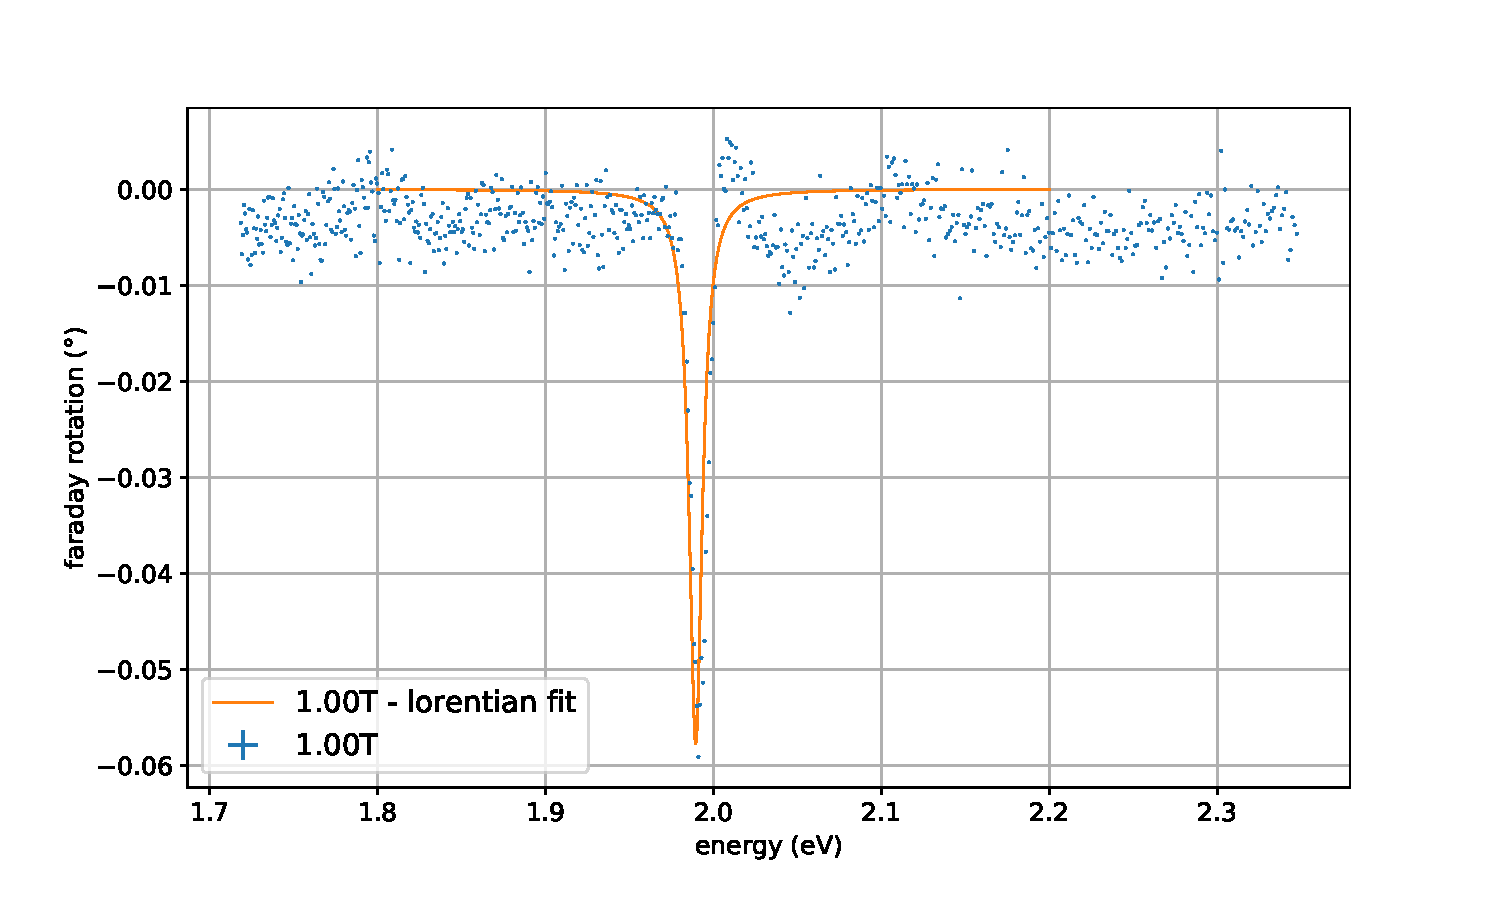
\includegraphics[width=1.0\textwidth]{plots/WS2_1000mT.pdf}
    \caption{}
    %label{fig_antibunch_background_comp}
    \end{subfigure}
    %\hfill
    \begin{subfigure}{0.47\textwidth}
        \centering
        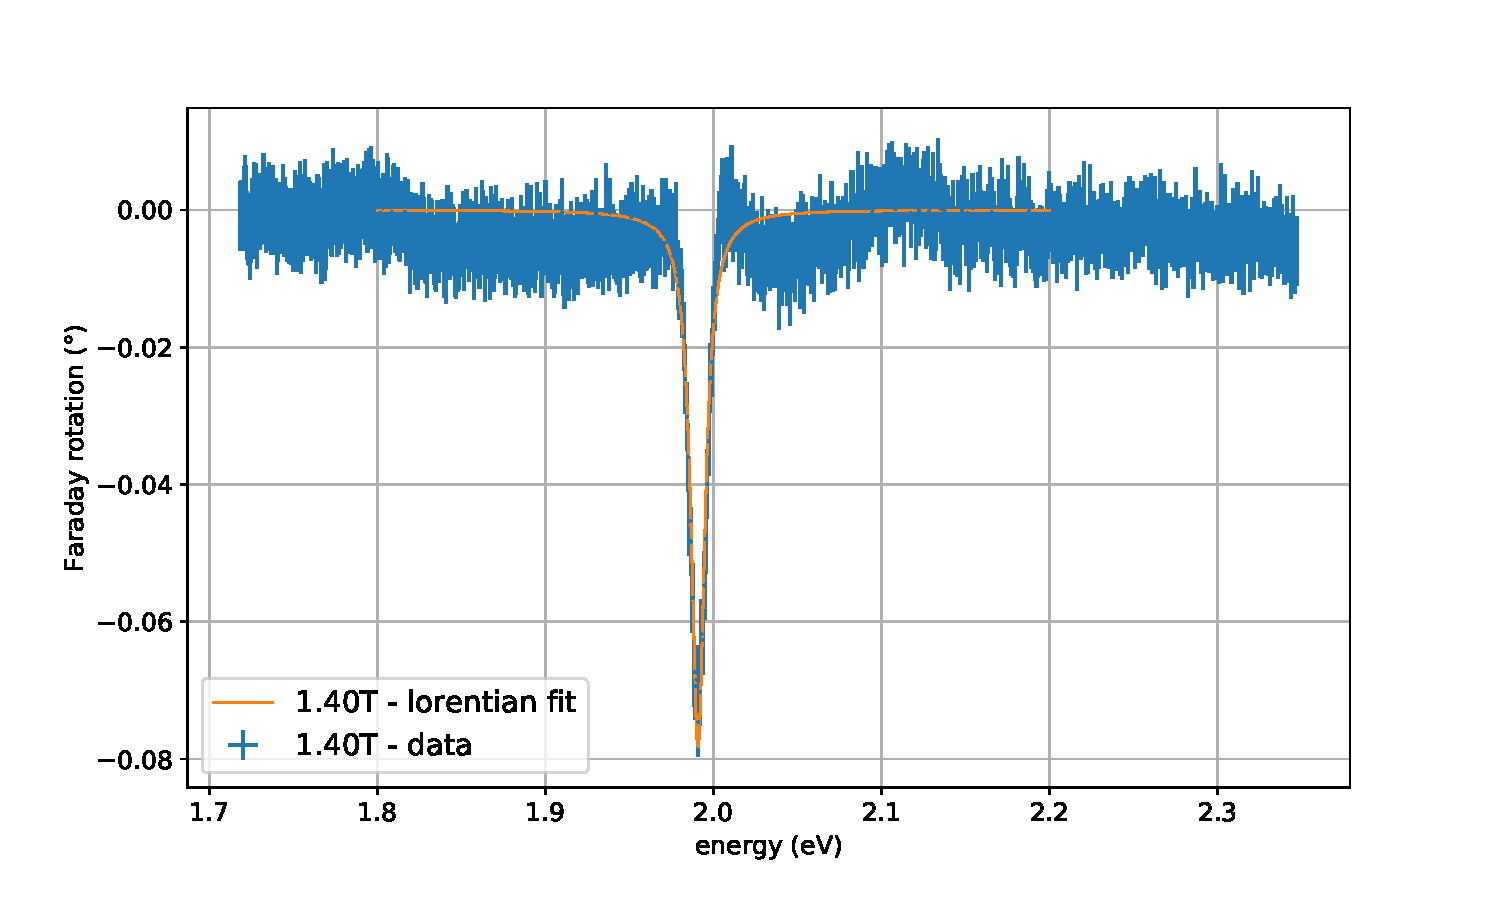
\includegraphics[width=\textwidth]{plots/WS2_1400mT.pdf}
        \caption{}
    \end{subfigure}
    \caption{a: Representation of WS$_2$ monolayer data points of the faraday rotation with external magnetic field of \SI{1.0}{\tesla} and lorentian fit. b: Same as a, but at \SI{1.4}{\tesla}.} %hoffe ok, dass der eine so doppelt ist
\end{figure}

	\printbibliography


\end{document}
